% ------------------------------------------------------------------------
% ------------------------------------------------------------------------
% Modelo UFSC para Trabalhos Academicos (tese de doutorado, dissertação de
% mestrado) utilizando a classe abntex2
%
% Autor: Alisson Lopes Furlani
% 	Modificações:
%	- 27/08/2019: Alisson L. Furlani, add pacote 'glossaries' para listas
% ------------------------------------------------------------------------
% ------------------------------------------------------------------------

\documentclass[
	% -- opções da classe memoir --
	12pt,				% tamanho da fonte
	%openright,			% capítulos começam em pág ímpar (insere página vazia caso preciso)
	oneside,			% para impressão no anverso. Oposto a twoside
	a4paper,			% tamanho do papel. 
	% -- opções da classe abntex2 --
	chapter=TITLE,		% títulos de capítulos convertidos em letras maiúsculas
	section=TITLE,		% títulos de seções convertidos em letras maiúsculas
	%subsection=TITLE,	% títulos de subseções convertidos em letras maiúsculas
	%subsubsection=TITLE,% títulos de subsubseções convertidos em letras maiúsculas
	% -- opções do pacote babel --
	english,			% idioma adicional para hifenização
	%french,				% idioma adicional para hifenização
	%spanish,			% idioma adicional para hifenização
	brazil				% o último idioma é o principal do documento
	]{abntex2}

\usepackage{setup/ufscthesisA4-alf}
%\addbibresource{aftertext/references.bib} % Seus arquivos de referências

%% ---
%% Filtering and Mapping Bibliographies
%% ---
%\DeclareSourcemap{
%	\maps[datatype=bibtex]{
%		% remove fields that are always useless
%		\map{
%			\step[fieldset=abstract, null]
%			\step[fieldset=pagetotal, null]
%		}
%		% remove URLs for types that are primarily printed
%%		\map{
%%			\pernottype{software}
%%			\pernottype{online}
%%			\pernottype{report}
%%			\pernottype{techreport}
%%			\pernottype{standard}
%%			\pernottype{manual}
%%			\pernottype{misc}
%%			\step[fieldset=url, null]
%%			\step[fieldset=urldate, null]
%%		}
%		\map{
%			\pertype{inproceedings}
%			% remove mostly redundant conference information
%			\step[fieldset=venue, null]
%			\step[fieldset=eventdate, null]
%			\step[fieldset=eventtitle, null]
%			% do not show ISBN for proceedings
%			\step[fieldset=isbn, null]
%			% Citavi bug
%			\step[fieldset=volume, null]
%		}
%	}
%}
%% ---

\newcommand{\sasize}{.9}
\newcommand{\annsize}{.7}
\newcommand{\figsize}{.6}

% ---
% Informações de dados para CAPA e FOLHA DE ROSTO
% ---
% FIXME Substituir 'Nome completo do autor' pelo seu nome.
\autor{Marcelo Salles Olinger}
% FIXME Substituir 'Título do trabalho' pelo título da trabalho.
\titulo{Predição de conforto térmico em escritórios ventilados naturalmente por meio de redes neurais artificiais}
% FIXME Substituir 'Subtítulo (se houver)' pelo subtítulo da trabalho.  
% Caso não tenha substítulo, comente a linha a seguir.
%\subtitulo{Subtítulo (se houver)}
% FIXME Substituir 'XXXXXX' pelo nome do seu
% orientador.
%\orientador{Prof. XXXXXX, Dr.}
% FIXME Se for orientado por uma mulher, comente a linha acima e descomente a linha a seguir.
\orientador[Orientadora]{Profa. Ana Paula Melo, Dra.}
% FIXME Substituir 'XXXXXX' pelo nome do seu
% coorientador. Caso não tenha coorientador, comente a linha a seguir.
\coorientador{Prof. Roberto Lamberts, Phd.}
% FIXME Se for coorientado por uma mulher, comente a linha acima e descomente a linha a seguir.
% \coorientador[Coorientadora]{XXXXXX, Dra.}
% FIXME Substituir 'XXXXXX' pelo nome do Coordenador do 
% programa/curso.
%\coordenador{Prof. XXXXXX, Dr.}
% FIXME Se for coordenadora mulher, comente a linha acima e descomente a linha a seguir.
\coordenador[Coordenadora]{Profa. Poliana Dias de Moraes, Dra.}
% FIXME Substituir '[ano]' pelo ano (ano) em que seu trabalho foi defendido.
\ano{2019}
% FIXME Substituir '[dia] de [mês] de [ano]' pela data em que ocorreu sua defesa.
\data{12 de setembro de 2019}
% FIXME Substituir 'Local' pela cidade em que ocorreu sua defesa.
\local{Florianópolis}
\instituicaosigla{UFSC}
\instituicao{Universidade Federal de Santa Catarina}
% FIXME Substituir 'Dissertação/Tese' pelo tipo de trabalho (Tese, Dissertação). 
\tipotrabalho{Dissertação}
% FIXME Substituir '[mestre/doutor] em XXXXXX' pela grau adequado.
\formacao{mestre em Engenharia Civil}
% FIXME Substituir '[mestrado/doutorado]' pelo nivel adequado.
\nivel{mestrado}
% FIXME Substituir 'Programa de Pós-Graduação em XXXXXX' pela curso adequado.
\programa{Programa de Pós-Graduação em Engenharia Civil}
% FIXME Substituir 'Campus XXXXXX ou Centro de XXXXXX' pelo campus ou centro adequado.
\centro{Campus Reitor João David Ferreira Lima}
\preambulo
{%
	\imprimirtipotrabalho~submetida~ao~\imprimirprograma~da~\imprimirinstituicao~para~a~obtenção~do~título~de~\imprimirformacao.
}
% ---

% ---
% Configurações de aparência do PDF final
% ---
% alterando o aspecto da cor azul
\definecolor{blue}{RGB}{41,5,195}
% informações do PDF
\makeatletter
\hypersetup{
     	%pagebackref=true,
		pdftitle={\@title}, 
		pdfauthor={\@author},
    	pdfsubject={\imprimirpreambulo},
	    pdfcreator={LaTeX with abnTeX2},
		pdfkeywords={ufsc, latex, abntex2}, 
		colorlinks=true,       		% false: boxed links; true: colored links
    	linkcolor=black,%blue,          	% color of internal links
    	citecolor=black,%blue,        		% color of links to bibliography
    	filecolor=black,%magenta,      		% color of file links
		urlcolor=black,%blue,
		bookmarksdepth=4
}
\makeatother
% ---
%\gls{q} \Gls{latex} \Glspl{formula} \acrshort{gcd} \acrlong{DCC} \acrfull{lcm}
% Abreviaturas
\newacronym{vn}{VN}{ventilação natural}
\newacronym{iea}{IEA}{Agência Internacional de Energia}
\newacronym{aivc}{AIVC}{\textit{Air Infiltration and Ventilation Centre}}
\newacronym{hvac}{HVAC}{\textit{heating, ventilating and air conditioning}}
\newacronym{pmv}{PMV}{voto predito médio}
\newacronym{ann}{ANN}{redes neurais artificiais}
\newacronym{svm}{MVS}{máquinas de vetores de suporte}
\newacronym{cfd}{CFD}{\textit{Computer Fluid Dynamics}}
\newacronym{afn}{AFN}{\textit{Airflow Network}}
\newacronym{ct}{CT}{capacidade térmica}
\newacronym{cp}{$C_p$}{coeficientes de pressão do vento}
\newacronym{cq}{$C_Q$}{coeficiente de fluxo mássico de ar}
\newacronym{cpeq}{$C_{p,eq}$}{coeficiente de pressão equivalente}
\newacronym{cd}{$C_d$}{coeficiente de descarga}
\newacronym{tpu}{TPU}{Universidade Politécnica de Tóquio}
\newacronym{paf}{PAF}{percentual de abertura na fachada}
\newacronym{fs}{FS}{fator solar}
\newacronym{as}{AS}{análise de sensibilidade}
\newacronym{ehf}{EHF}{fração de horas de desconforto por calor}
\newacronym{ach}{ACH}{trocas de ar por hora}
\newacronym{rmse}{RMSE}{raiz quadrada do erro quadrático médio}
\newacronym{nrmse}{NRMSE}{raiz quadrada do erro quadrático médio normalizada}
\newacronym{r2}{R$^2$}{coeficiente de determinação}
\newacronym{abse}{MAE}{erro absoluto médio}
\newacronym{ae95}{AE95}{erro absoluto do 95º percentil}
\newacronym{ma}{MA}{método analítico}
\newacronym{inic}{INI-C}{Proposta de Instrução Normativa do Inmetro para a Classe de Eficiência Energética de Edificações Comerciais, de Serviços e Públicas}
 

%List of Symbols
\newglossaryentry{px}{	% how the symbol will be called in the text \gls{x}
	type=symbols,		% set the glossary entry type as "symbol"
	name={\ensuremath{P_x}},	
	description={pressão estática do ar em um ponto da fachada do edifício},
	user1=\unexpanded{\si{\pascal}}
}
\newglossaryentry{p0}{	% how the symbol will be called in the text \gls{x}
type=symbols,		% set the glossary entry type as "symbol"
name={\ensuremath{P_{\infty}}},	
description={pressão estática de referência do ar},
user1=\unexpanded{\si{\pascal}}
}
\newglossaryentry{pd}{	% how the symbol will be called in the text \gls{x}
type=symbols,		% set the glossary entry type as "symbol"
name={\ensuremath{P_d}},	
description={pressão dinâmica do ar},
user1=\unexpanded{\si{\pascal}}
}
\newglossaryentry{rho}{	% how the symbol will be called in the text \gls{x}
type=symbols,		% set the glossary entry type as "symbol"
name={\ensuremath{\rho}},	
description={densidade do ar},
user1=\unexpanded{\si{\kilogram/\cubic\meter}}
}
\newglossaryentry{vref}{	% how the symbol will be called in the text \gls{x}
type=symbols,		% set the glossary entry type as "symbol"
name={\ensuremath{V_{\infty}}},	
description={velocidade de referência do vento},
user1=\unexpanded{\si{\meter/\second}}
}
\newglossaryentry{tinf}{	% how the symbol will be called in the text \gls{x}
type=symbols,		% set the glossary entry type as "symbol"
name={\ensuremath{T_{inf}}},	
description={limite inferior da temperatura operativa para 80\% de aceitabilidade no conforto térmico},
user1=\unexpanded{\si{\celsius}}
}
\newglossaryentry{tsup}{	% how the symbol will be called in the text \gls{x}
type=symbols,		% set the glossary entry type as "symbol"
name={\ensuremath{T_{sup}}},	
description={limite superior da temperatura operativa para 80\% de aceitabilidade no conforto térmico},
user1=\unexpanded{\si{\celsius}}
}
\newglossaryentry{tm}{	% how the symbol will be called in the text \gls{x}
type=symbols,		% set the glossary entry type as "symbol"
name={\ensuremath{T_m}},	
description={temperatura média do ar externo},
user1=\unexpanded{\si{\celsius}}
}
\newglossaryentry{tssup}{	% how the symbol will be called in the text \gls{x}
type=symbols,		% set the glossary entry type as "symbol"
name={\ensuremath{timesteps_{sup}}},	
description={número de \textit{timesteps} em que há ocupação na zona térmica e a temperatura operativa ultrapassa o limite superior determinado pelo método adaptativo}%,
%user1= {-} %\unexpanded{\si{\celsius}}
}
\newglossaryentry{tsocup}{	% how the symbol will be called in the text \gls{x}
type=symbols,		% set the glossary entry type as "symbol"
name={\ensuremath{timesteps_{sup}}},	
description={número de \textit{timesteps} em que há ocupação na zona térmica}%,
%user1= {-} %\unexpanded{\si{\celsius}}
}

\newglossaryentry{tsupv}{	% how the symbol will be called in the text \gls{x}
	type=symbols,		% set the glossary entry type as "symbol"
	name={\ensuremath{T_{sup,v}}},	
	description={temperatura limite superior na faixa de conforto, considerando-se a velocidade do ar},
	user1= \unexpanded{\si{\celsius}}
}
\newglossaryentry{tvar}{	% how the symbol will be called in the text \gls{x}
type=symbols,		% set the glossary entry type as "symbol"
name={\ensuremath{T_{v_{ar}}}},	
description={margem extra de temperatura permitida pela consideração da velocidade do ar},
user1= \unexpanded{\si{\celsius}}
}
\newglossaryentry{rmsecp}{	% how the symbol will be called in the text \gls{x}
type=symbols,		% set the glossary entry type as "symbol"
name={\ensuremath{RMSE_{Cp}}},
description={RMSE das diferenças entre os valores dos Cp's obtidos pela base da TPU e obtidos pelo MA},
user1= {-}%\unexpanded{\si{\celsius}}
}
\newglossaryentry{alphaj}{	% how the symbol will be called in the text \gls{x}
type=symbols,		% set the glossary entry type as "symbol"
name={\ensuremath{\alpha_j}},	
description={ângulo de incidência do vento  sobre a fachada, e tem valor igual a $30 \cdot j$},
user1= \ensuremath{^{\circ}}
}
\newglossaryentry{meancptpu}{	% how the symbol will be called in the text \gls{x}
type=symbols,		% set the glossary entry type as "symbol"
name={\ensuremath{\overline{Cp}^{TPU}_{f_i,\alpha_j,p_k}}},	
description={valor do Cp disponibilizado pela base de dados da TPU para a fachada $i$ de uma edificação, para o ângulo de incidência do vento igual a $\alpha_j$, no ponto $k$}, %\glsname{tpu} \glsname{alphaj}}
user1= {-}%\unexpanded{\si{\celsius}}
}
\newglossaryentry{cpma}{	% how the symbol will be called in the text \gls{x}
type=symbols,		% set the glossary entry type as "symbol"
name={\ensuremath{Cp^{MA}_{f_i,\alpha_j}}},	
description={Cp calculado pelo MA para a fachada de uma edificação com proporções iguais às da fachada $i$, para o ângulo de incidência do vento igual a $\alpha_j$}, %\glsname{ma} \glsname{alphaj}
user1= {-}%\unexpanded{\si{\celsius}}
}
\newglossaryentry{fi}{	% how the symbol will be called in the text \gls{x}
type=symbols,		% set the glossary entry type as "symbol"
name={\ensuremath{f_i}},	
description={fachada $i$ da edificação avaliada},
user1= {-}%\unexpanded{\si{\celsius}}
}
\newglossaryentry{m}{	% how the symbol will be called in the text \gls{x}
type=symbols,		% set the glossary entry type as "symbol"
name={\ensuremath{\dot{m}_{i,j}}},	
description={fluxo de ar entre os pontos $i$ e $j$, quando a porta/janela está aberta},
user1=\unexpanded{\si{\kilogram/\second}}
}
\newglossaryentry{n}{	% how the symbol will be called in the text \gls{x}
type=symbols,		% set the glossary entry type as "symbol"
name={\ensuremath{\dot{n}_{i,j}}},	
description={fluxo de ar entre os pontos $i$ e $j$, quando a porta/janela está fechada},
user1=\unexpanded{\si{\kilogram/\second}}
}
\newglossaryentry{theta}{	% how the symbol will be called in the text \gls{x}
	type=symbols,		% set the glossary entry type as "symbol"
	name={\ensuremath{\Theta}},	
	description={fração de abertura da porta/janela},
	user1={-} %\unexpanded{\si{\kilogram/\second}}
}
\newglossaryentry{height}{	% how the symbol will be called in the text \gls{x}
type=symbols,		% set the glossary entry type as "symbol"
name={\ensuremath{H}},	
description={altura da abertura},
user1= \unexpanded{\si{\meter}}
}
\newglossaryentry{width}{	% how the symbol will be called in the text \gls{x}
type=symbols,		% set the glossary entry type as "symbol"
name={\ensuremath{W}},	
description={largura da abertura},
user1= \unexpanded{\si{\meter}}
}
\newglossaryentry{piz}{	% how the symbol will be called in the text \gls{x}
type=symbols,		% set the glossary entry type as "symbol"
name={\ensuremath{P_{i(z)}}},	
description={pressão de ar no ponto $i$, altura $z$},
user1= \unexpanded{\si{\pascal}}
}
\newglossaryentry{cqq}{	% how the symbol will be called in the text \gls{x}
type=symbols,		% set the glossary entry type as "symbol"
name={\ensuremath{C_Q}},	
description={coeficiente de fluxo mássico de ar},
user1={-} %\unexpanded{\si{\kilogram/\second}}
}
\newglossaryentry{cdd}{	% how the symbol will be called in the text \gls{x}
type=symbols,		% set the glossary entry type as "symbol"
name={\ensuremath{C_d}},	
description={coeficiente de descarga da abertura},
user1={-} %\unexpanded{\si{\kilogram/\second}}
}
\newglossaryentry{cpp}{	% how the symbol will be called in the text \gls{x}
type=symbols,		% set the glossary entry type as "symbol"
name={\ensuremath{C_p}},	
description={coeficiente de pressão},
user1={-} %\unexpanded{\si{\kilogram/\second}}
}
\newglossaryentry{cppeq}{	% how the symbol will be called in the text \gls{x}
type=symbols,		% set the glossary entry type as "symbol"
name={\ensuremath{C{_p,eq}}},	
description={coeficiente de pressão equivalente},
user1={-} %\unexpanded{\si{\kilogram/\second}}
}
\newglossaryentry{exp}{	% how the symbol will be called in the text \gls{x}
type=symbols,		% set the glossary entry type as "symbol"
name={\ensuremath{exp}},	
description={ expoente de fluxo de massa de ar},
user1={-} %\unexpanded{\si{\kilogram/\second}}
}
\newglossaryentry{pzn}{	% how the symbol will be called in the text \gls{x}
type=symbols,		% set the glossary entry type as "symbol"
name={\ensuremath{P_{zn}}},	
description={pressão do ar na zona térmica analisada},
user1=\unexpanded{\si{\pascal}}
}
\newglossaryentry{pi}{	% how the symbol will be called in the text \gls{x}
type=symbols,		% set the glossary entry type as "symbol"
name={\ensuremath{P_i}},	
description={pressão do ar na zona térmica, ligada pela porta $i$},
user1=\unexpanded{\si{\pascal}}
}
\newglossaryentry{np}{	% how the symbol will be called in the text \gls{x}
type=symbols,		% set the glossary entry type as "symbol"
name={\ensuremath{N_P}},	
description={número de portas que se conectam à zona térmica}
}
\newglossaryentry{nj}{	% how the symbol will be called in the text \gls{x}
type=symbols,		% set the glossary entry type as "symbol"
name={\ensuremath{N_J}},	
description={número de janelas que se conectam à zona térmica}
}
\newglossaryentry{li}{	% how the symbol will be called in the text \gls{x}
type=symbols,		% set the glossary entry type as "symbol"
name={\ensuremath{L_i}},	
description={perímetro da porta $i$},
user1= \unexpanded{\si{\meter}}
}
\newglossaryentry{area}{	% how the symbol will be called in the text \gls{x}
type=symbols,		% set the glossary entry type as "symbol"
name={\ensuremath{A_j}},	
description={área da janela $j$},
user1= \unexpanded{\si{\square\meter}}
}
\newglossaryentry{pext}{	% how the symbol will be called in the text \gls{x}
type=symbols,		% set the glossary entry type as "symbol"
name={\ensuremath{P_{ext}}},	
description={pressão do ar no ambiente externo},
user1=\unexpanded{\si{\pascal}}
}
\newglossaryentry{cpj}{	% how the symbol will be called in the text \gls{x}
type=symbols,		% set the glossary entry type as "symbol"
name={\ensuremath{C_{p,j}}},	
description={Cp na superície da janela $j$},
user1={-} %\unexpanded{\si{\kilogram/\second}}
}
\newglossaryentry{deltamet}{	% how the symbol will be called in the text \gls{x}
type=symbols,		% set the glossary entry type as "symbol"
name={\ensuremath{\delta_{met}}},	
description={espessura da camada limite para o perfil de vento na estação meteorológica},
user1=\unexpanded{\si{\meter}}
}
\newglossaryentry{alphamet}{	% how the symbol will be called in the text \gls{x}
type=symbols,		% set the glossary entry type as "symbol"
name={\ensuremath{\alpha_{met}}},	
description={expoente para o perfil de vento na estação meteorológica},
user1={-} %\unexpanded{\si{\kilogram/\second}}
}
\makenoidxglossaries 

% ---

% ---
% compila o indice
% ---
\makeindex
% ---

% ----
% Início do documento
% ----
\begin{document}

% Seleciona o idioma do documento (conforme pacotes do babel)
%\selectlanguage{english}
\selectlanguage{brazil}

% Retira espaço extra obsoleto entre as frases.
\frenchspacing 

% Espaçamento 1.5 entre linhas
\OnehalfSpacing

% Corrige justificação
%\sloppy

% ----------------------------------------------------------
% ELEMENTOS PRÉ-TEXTUAIS
% ----------------------------------------------------------
% \pretextual %a macro \pretextual é acionado automaticamente no início de \begin{document}
% ---
% Capa, folha de rosto, ficha bibliografica, errata, folha de apróvação
% Dedicatória, agradecimentos, epígrafe, resumos, listas
% ---
% ---
% Capa
% ---
\imprimircapa
% ---

% ---
% Folha de rosto
% (o * indica que haverá a ficha bibliográfica)
% ---
\imprimirfolhaderosto*
% ---

% ---
% Inserir a ficha bibliografica
% ---
% http://ficha.bu.ufsc.br/
\begin{fichacatalografica}
	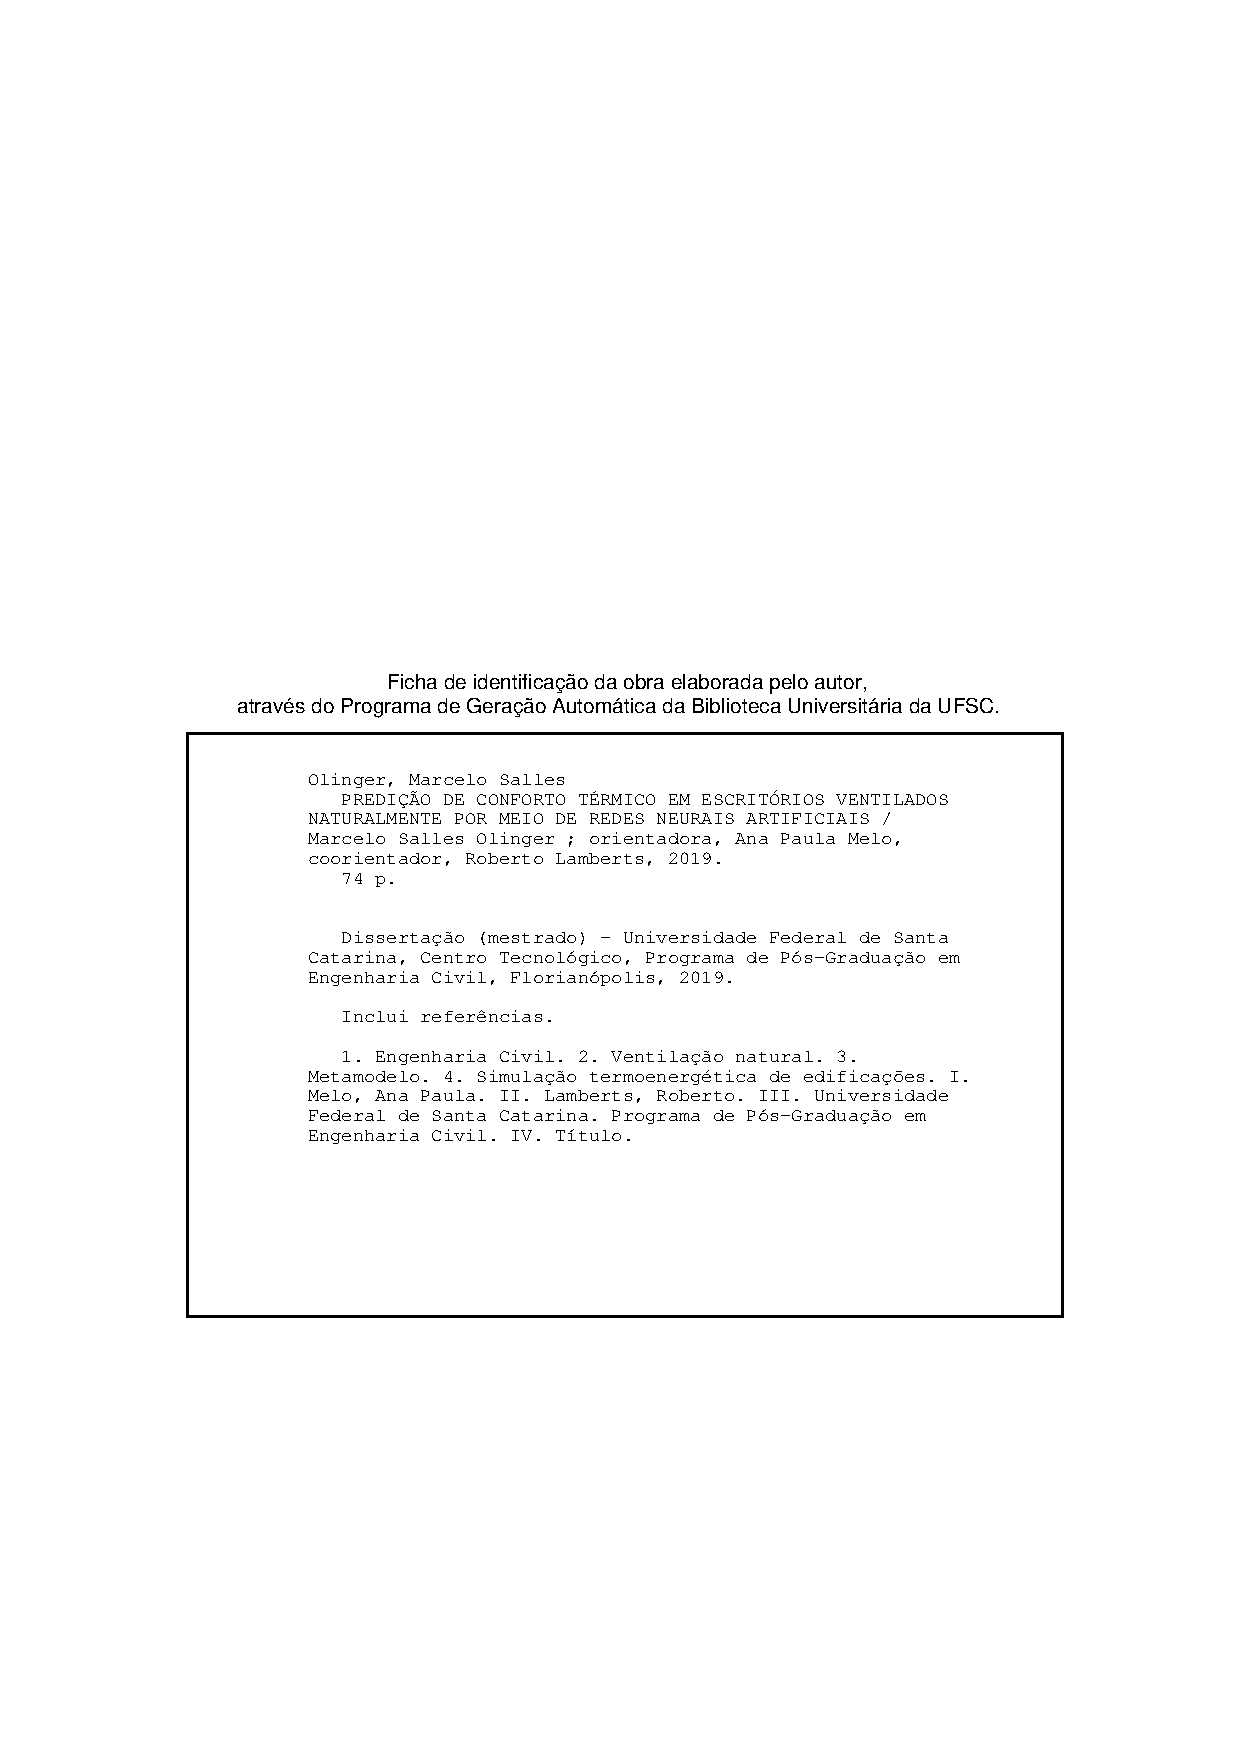
\includepdf{beforetext/Ficha_Catalografica.pdf}
\end{fichacatalografica}
% ---

% ---
% Inserir folha de aprovação
% ---
\begin{folhadeaprovacao}
	\OnehalfSpacing
	\centering
	\imprimirautor\\%
	\vspace*{10pt}		
	\textbf{\imprimirtitulo}%
	\ifnotempty{\imprimirsubtitulo}{:~\imprimirsubtitulo}\\%
	%		\vspace*{31.5pt}%3\baselineskip
	\vspace*{\baselineskip}
	%\begin{minipage}{\textwidth}
	O presente trabalho em nível de \imprimirnivel~foi avaliado e aprovado por banca examinadora composta pelos seguintes membros:\\
	%\end{minipage}%
	\vspace*{\baselineskip}
	Prof. Saulo Guths, Dr.\\
	Universidade Federal de Santa Catarina\\
	\vspace*{\baselineskip}
	Prof. Martin Gabriel Ordenes Mizgier, Dr.\\
	Universidade Federal de Santa Catarina\\
	\vspace*{\baselineskip}
	Facundo Bre, Dr.\\
	Universidad Nacional del Litoral, Argentina\\
	\vspace*{2\baselineskip}
	\begin{minipage}{\textwidth}
		Certificamos que esta é a \textbf{versão original e final} do trabalho de conclusão que foi julgado adequado para obtenção do título de \imprimirformacao.\\
	\end{minipage}
	%    \vspace{-0.7cm}
	\vspace*{\fill}
	\assinatura{\OnehalfSpacing\imprimircoordenador \\ \imprimircoordenadorRotulo~do Programa}
	\vspace*{\fill}
	\assinatura{\OnehalfSpacing\imprimirorientador \\ \imprimirorientadorRotulo}
	%	\ifnotempty{\imprimircoorientador}{
	%	\assinatura{\imprimircoorientador \\ \imprimircoorientadorRotulo \\
	%		\imprimirinstituicao~--~\imprimirinstituicaosigla}
	%	}
	% \newpage
	\vspace*{\fill}
	\imprimirlocal, \imprimirdata.
\end{folhadeaprovacao}
% ---

% ---
% Dedicatória
% ---
%\begin{dedicatoria}
%	\vspace*{\fill}
%	\noindent
%	\begin{adjustwidth*}{}{5.5cm}     
%		Este trabalho é dedicado aos meus colegas de classe e aos meus queridos pais.
%	\end{adjustwidth*}
%\end{dedicatoria}
% ---

% ---
% Agradecimentos
% ---
\begin{agradecimentos}
	Muito obrigado à família, amigos e colegas! 
\end{agradecimentos}
% ---

% ---
% Epígrafe
% ---
\begin{epigrafe}
	\vspace*{\fill}
	\begin{flushright}
		\textit{``All models are wrong, but some are useful.''\\
			(George E. P. Box)}
	\end{flushright}
\end{epigrafe}
% ---

% ---
% RESUMOS
% ---

% resumo em português
\setlength{\absparsep}{18pt} % ajusta o espaçamento dos parágrafos do resumo
\begin{resumo}
	\SingleSpacing
	O condicionamento de ar para resfriamento de edificações é responsável por parcela significativa do consumo energético no mundo, e isso tende a aumentar nas próximas décadas. Uma solução para a mitigação do aumento no consumo de energia para resfriamento de ar é uso de ventilação natural (VN). 
	A VN é uma técnica de resfiramento passivo com um potencial significativo de aplicação em países de clima quente. 
	Apesar de seu pontencial de aplicabilidade, o uso de VN em edifícios de escritórios
	vem diminuindo gradualmente no Brasil, pois edificações de escritórios recentes vêm sendo projetadas exclusivamente com sistemas de condicionamento de ar.	
	Para que seja aplicada de forma efetiva, é importante que a VN seja concebida desde a fase inicial de projeto. Durante a fase inicial de projeto, há pouco detalhamento relacionado ao projeto arquitetônico, e há necessidade de agilidade nas tomadas de decisão.
	Diante deste cenário, uma ferramenta capaz de estimar o conforto térmico em edificações de forma simples e rápida pode ser de grande utilidade.	
	O objetivo deste estudo é desenvolver um metamodelo de rede neural artificial capaz de estimar o conforto térmico em edificações de escritórios ventilados naturalmente. 
	O indicador de conforto térmico utilizado é a fração de horas do ano em que há desconforto térmico por calor no ambiente (EHF), de acordo com o método adaptativo da ASHRAE Standard 55 (2017), para 80\% de aceitabilidade entre os ocupantes.	
	O metamodelo é desenvolvido a partir de uma base de dados de simulações termoenergéticas obtidas através do programa computacional EnergyPlus. Os modelos que compõem a base de dados foram definidos a partir das características comumente encontradas em edificações de escritórios da cidade de São Paulo. A definição dos parâmetros variados no desenvolvimento dos modelos é estabelecida através da análise de sensibilidade global de Sobol.	
	O treinamento da rede neural artificial é realizado com uma base de dados de 100.000 simulações termoenergéticas, amostradas pelo método de amostragem do hipercubo latino. 
	O desempenho do metamodelo foi avaliado para uma amostra de validação com 20.000 casos, e obteve resultados de EHF com um erro absoluto médio igual a 0,009, e um erro absoluto do 95º percentil igual a 0,024.	
	O metamodelo desenvolvido foi capaz de estimar o conforto térmico em edificações de escritórios ventilados naturalmente para a cidade de São Paulo com resultados próximos aos obtidos pelo programa de simulação computacional EnergyPlus.
	Esse metamodelo pode ser utilizado por projetistas como uma ferramenta de fácil aplicação no suporte à tomada de decisão em fases iniciais de projeto.
	
	\textbf{Palavras-chave}: Ventilação natural. Metamodelo. Simulação termoenergética de edificações.
\end{resumo}

% resumo em inglês
\begin{resumo}[Abstract]
	\SingleSpacing
	\begin{otherlanguage*}{english}
		Energy demand in the world for air cooling in buildings is significant, and it is expected to increase in the next decades.
		Natural ventilation (NV) could be a solution to mitigate energy use for air cooling, since it is a passive cooling strategy with significant potential for hot climates.
		Despite its potential, the use of NV has been decreasing in recent years for office buildings in Brazil, since the design of buildings with air conditioning prevails.		
		It is important to conceive the use of NV since early-design phases of the building to guarantee its effectiveness.
		During early-design phases, there are uncertainties related to the many construction parameters, and the decision process has to occur fast.
		Given the current scenario, the development of a surrogate model capable of estimate thermal comfort in buildings in a simple and fast way could be of great use.		
		The aim of this study is to develop an artificial neural network model to estimate thermal comfort in naturally ventilated office buildings.
		The annual fraction of occupied hours within the thermal zone with operative temperatures above the upper limit of ASHRAE's Standards 55 (2017) adaptive model, for 80\% of acceptability, is used as a thermal comfort index.		
		The surrogate model is developed from a data set of building performance simulations, using the software EnergyPlus.
		Simulation models were defined based on a database of naturally ventilated office buildings in the city of São Paulo.
		The variables used as inputs in the surrogate model are defined by Sobol's sensitivity analysis.		
		From data of 100,000 simulations, sampled by Latin hypercube sampling method, the neural network was trained.
		The performance of the surrogate model was measured with a validation data set of 20,000 cases.
		The mean absolute error for the fraction of hours outside ASHRAE's Standards 55 (2017) adaptive model limits for the validation data set was 0,009, and the absolute error of the 95$^{th}$ percentile was 0,024.		
		The final surrogate model achieved estimates for thermal comfort in naturally ventilated office buildings in the city of São Paulo with results close to the simulations developed on the software EnergyPlus. This surrogate model can be used by building designers as a simple tool to support decision making in early-design phases.
		
		\textbf{Keywords}: Natural ventilation. Surrogate model. Building performance simulation.
	\end{otherlanguage*}
\end{resumo}

%% resumo em francês 
%\begin{resumo}[Résumé]
% \begin{otherlanguage*}{french}
%    Il s'agit d'un résumé en français.
% 
%   \textbf{Mots-clés}: latex. abntex. publication de textes.
% \end{otherlanguage*}
%\end{resumo}
%
%% resumo em espanhol
%\begin{resumo}[Resumen]
% \begin{otherlanguage*}{spanish}
%   Este es el resumen en español.
%  
%   \textbf{Palabras clave}: latex. abntex. publicación de textos.
% \end{otherlanguage*}
%\end{resumo}
%% ---

{%hidelinks
	\hypersetup{hidelinks}
	% ---
	% inserir lista de ilustrações
	% ---
	\pdfbookmark[0]{\listfigurename}{lof}
	\listoffigures*
	\cleardoublepage
	% ---
	
	% ---
	% inserir lista de quadros
	% ---
%	\pdfbookmark[0]{\listofquadrosname}{loq}
%	\listofquadros*
%	\cleardoublepage
	% ---
	
	% ---
	% inserir lista de tabelas
	% ---
	\pdfbookmark[0]{\listtablename}{lot}
	\listoftables*
	\cleardoublepage
	% ---
	
	% ---
	% inserir lista de abreviaturas e siglas (devem ser declarados no preambulo)
	% ---
	\imprimirlistadesiglas
	% ---
	
	% ---
	% inserir lista de símbolos (devem ser declarados no preambulo)
	% ---
	\imprimirlistadesimbolos
	% ---
	
	% ---
	% inserir o sumario
	% ---
	\pdfbookmark[0]{\contentsname}{toc}
	\tableofcontents*
	\cleardoublepage
	
}%hidelinks
% ---
% ---

% ----------------------------------------------------------
% ELEMENTOS TEXTUAIS
% ----------------------------------------------------------
\textual

% ---
% 1 - Introdução
% ---
% ----------------------------------------------------------
\chapter{Introdução}
\label{chapter:introducao}

De acordo com a \acrlong{iea} \cite{IEA2018a}, no ano de 2017 o setor de edificações representou mais de 30\% do consumo final total de energia no mundo. 
O relatória da \citeonline{IEA2018} aponta que a demanda por energia destinada ao resfriamento de ar em edificações mais que triplicou do ano de 1990 a 2016 e, se não houver mudanças no cenário atual, estima-se que essa demanda mais que triplicará até o ano de 2050, representando 37\% do aumento no consumo de eletricidade em edificações. Isso corresponderá a 11,5\% do consumo de energia total em edificações comerciais. 
O potencial de aumento na demanda por energia destinada ao resfriamento de ar em países de clima quente é ainda mais expressivo. Das 2,8 bilhões de pessoas que vivem nas partes mais quentes do mundo hoje, apenas 8\% possuem sistema de condicionamento de ar \cite{IEA2018}. No Brasil, a parcela do resfriamento de ar nas cargas de pico das redes elétricas em 2016 correspondia a 7,6\% do total, e a estimativa, considerando-se o cenário base, é de que essa parcela represente 30,8\% da carga de pico até o ano de 2050 \cite{IEA2018}. 
%No Brasil, desde 2009 o INMETRO possui um programa de etiquetagem de edificações voltado para padrões de eficiência energética de edificações \cite{BRASIL2009}.

Esse contexto evidencia a necessidade de medidas mitigadoras relacionadas ao consumo energético destinado ao resfriamento de edificações. O uso de técnicas de resfriamento passivo, como a \acrfull{vn}, pode ser uma solução. O resfriamento passivo é um conjunto de técnicas sustentáveis para resfriar edifícios por meios naturais \cite{Samani2016}, que consiste em qualquer sistema que busca minimizar, ou eliminar, se possível, o uso de sistemas de condicionamento de ar, com o objetivo de reduzir as altas temperaturas internas e o consumo de energia para resfriamento, proporcionando conforto térmico aos ocupantes.

Técnicas de \acrshort{vn} são encontradas ao longo de toda a história na arquitetura vernacular \cite{Pesic2018}, e hoje vêm sendo atualizadas de acordo com novos estudos no campo de conforto térmico e projetos sustentáveis de edificações.
Além de assegurar a qualidade do ar, a \acrshort{vn} promove o resfriamento da edificação, proporcionando conforto térmico aos usuários quando as condições do clima externo são favoráveis \cite{Yao2009}.

Apesar de um quinto da energia elétrica brasileira ser destinada a edificações comerciais, de serviços e públicas \cite{EPE2018}, o uso de \acrshort{vn} em edifícios de escritórios vem diminuindo gradualmente no Brasil. De acordo com \citeonline{Alves2017}, apesar do uso de sistemas de condicionamento de ar e iluminação mais eficientes, edifícios da cidade de Belo Horizonte construídos a partir dos anos 2000 tendem a ser os maiores consumidores de energia, por não adotarem estratégias de resfriamento passivo.

Para que o conforto térmico dos usuários seja garantido sem um consumo significativo de energia, é importante entender como ocorrem as variações térmicas em um edifício antes de construí-lo. Análises durante os estágios iniciais de projeto de uma edificação com \acrshort{vn} apontam decisões fundamentais para o desempenho térmico. No estágio inicial de projeto, o potencial de otimização é significativo, e nesta etapa qualquer estimativa do conforto e desempenho energético da edificação pode refletir nas tomadas de decisão \cite{Belleri2014, Roetzel2014}.

O método mais avançado de se estimar o desempenho termoenergético de edificações atualmente é por meio de simulações computacionais. No entanto, esse processo exige o conhecimento técnico de um especialista, pois simulações termoenergéticas dinâmicas requerem modelos detalhados e enfrentam diversos problemas, associados principalmente a informações necessárias para dados de entrada do modelo processado \cite{Corgnati2013}. No contexto brasileiro, a análise do desempenho térmico de edificações por meio de simulações computacionais é uma medida relevante, pois, assim como em outros países em desenvolvimento, a falta de acessibilidade a dados relacionados a padrões de consumo de energia e atributos físicos e operacionais de edifícios de escritório dificulta as análises a partir de bancos de dados \cite{Alves2018}. Uma alternativa para contornar essas questões é o desenvolvimento de modelos a partir de simulações computacionais, os metamodelos. Por meio de metamodelos é possível se obter resultados próximos aos de simulações complexas de desempenho energético.

Metamodelos para eficiência energética de edificações podem ser desenvolvidos a partir de diferentes métodos \cite{Ostergard2018}. A solução mais apropriada depende do contexto e propósitos de cada aplicação.
\citeonline{Versage2015} foi capaz de estimar as cargas térmicas de edificações comerciais através de diferentes métodos de metamodelagem.
\citeonline{Melo2016} desenvolveram um modelo de \acrfull{ann} para estimar graus hora de resfriamento e cargas térmicas de aquecimento e resfriamento em edificações residenciais.
O desenvolvimento de um metamodelo de máquina de vetores de suporte capaz de estimar conforto térmico em edificações comerciais foi proposto por \citeonline{Rackes2016}. Voltado principalmente a tipologias de escolas, o metamodelo estima a fração de horas em desconforto por calor dos ocupantes ao longo do ano.
%
%A \acrshort{vn} em edificações apresenta comportamentos complexos e a avaliação do seu potencial de resfriamento faz-se necessária desde a fase inicial de projeto. Possibilitar esse tipo de análise de forma simples e rápida é fundamental nas tomadas de decisão em projetos de edificações e na aplicação de políticas públicas voltadas à eficiência energética. Por meio de ferramentas de aprendizagem automática, surge a oportunidade de se desenvolver metamodelos capazes de obter resultados de conforto térmico em edificações.

O consumo de energia para resfriamento de edificações é expressivo no mundo, e a expectativa é de que a demanda por energia continue crescendo nas próximas décadas, principalmente em países de climas quentes.
Neste contexto, o uso de técnicas de \acrfull{vn} apresenta-se como uma solução para mitigar o uso de condicionamento de ar.
Entretanto, o desempenho térmico das edificações apresenta fenômenos termofísicos complexos, fazendo com que estimativas de conforto térmico devam ser consideradas preferencialmente desde as etapas iniciais de projeto. 	
Na busca por uma ferramenta capaz de auxiliar projetistas de maneira rápida e simples, surge a possibilidade de utilizar-se metamodelos.
Portanto, este trabalho apresenta o desenvolvimento de um metamodelo capaz de estimar o conforto térmico em edifícios de escritórios ventilados naturalmente.

\section{Objetivos}
\subsection{Objetivo geral}

O objetivo deste estudo é desenvolver um metamodelo capaz de estimar o conforto térmico em edifícios de escritórios ventilados naturalmente.

\subsection{Objetivos específicos}

Dentre os objetivos específicos deste trabalho, destacam-se:

\begin{itemize}
	\item Identificar as características construtivas encontradas em edifícios de escritórios ventilados naturalmente na cidade de São Paulo;
	\item Desenvolver um modelo de simulação termoenergética simplificado, com apenas uma zona térmica, capaz de representar as trocas térmicas de uma sala em um edifício de escritórios;
	\item Definir as variáveis com maior e menor influência no desempenho térmico dos edifícios ventilados naturalmente.
\end{itemize}
% ---

% ---
% 2 - Capítulo 2
% ---
\include{chapters/revisao}
% ---

% ---
% 3 - Capítulo 3
% ---
\chapter{Metodologia}
\label{chapter:metodologia}

\section{Definição dos parâmetros de entrada e saída}

\subsection{Parâmetros de entrada}\label{subsec:par}

A princípio, a definição dos parâmetros adotados para gerar a base de dados de simulações para o desenvolvimento do metamodelo foram obtidos a partir do banco de dados com 153 edificações de escritórios com \acrfull{vn} disponibilizado por \citeonline{Neves2019}.  		
Dentre as informações  disponíveis no banco de dados, obtém-se:

\begin{itemize}
	\item orientação solar do edifício;
	\item número de pavimentos;
	\item forma dos pavimentos e das salas;
	\item áreas das salas;  % dos pavimentos e
	\item altura do pé-direito das salas;
	\item relações entre as dimensões dos pavimentos e entre as dimensões das salas;
	\item absortância das paredes externas; % 0.2 - 0.8
	%			\item espessura das paredes externas;
	\item cor da cobertura;
	\item tipo de vidro nas janelas;
	\item tipo de esquadria;
	\item fator de abertura das janelas;
	%			\item altura das esquadrias;
	\item \acrfull{paf};  % 0 - 80
	\item tipo de sombreamento;  % 0 - 80
	\item tipo de estratégia de \acrlong{vn} (unilateral ou cruzada).
\end{itemize} 

Os valores desses parâmetros foram observados através de suas distribuições de ocorrência. Desta forma definiu-se os limites mínimos e máximos para o desenvolvimento das simulações termoenergéticas, com parâmetros variando de acordo com o que se encontra comumente em edifícios reais. Como as edificações do banco de dados localizam-se na cidade de São Paulo, esse foi o clima para qual o metamodelo foi desenvolvido.

Certas informações não estão disponibilizadas pelo banco de dados analisado, como algumas relacionadas às propriedades termofísicas dos materiais da envoltória, às densidades de potência de iluminação e equipamentos, e aos padrões e taxas de ocupação. Frente a essa limitação, os valores desses parâmetros foram definidos a partir da \acrlong{inic} \cite{INIC}. %, através da Tabela 4.1, da Tabela A.1 do anexo A e da Tabela B.I.1 do anexo B.  % Hora início e fim: 8 - 18,  INI-C

A Tabela \ref{table:paramconst} apresenta os parâmetros que mantiveram-se com valores constantes no desenvolvimento do trabalho. Esses valores foram escolhidos a partir do que é apresentado na \citeonline{INIC} para a simulação das edificações nas condições de referência. A cobertura tem suas propriedades termofísicas baseadas na consideração de uma laje de concreto de 10 cm de espessura e telha de fibrocimento, separadas por uma câmara de ar. O padrão de ocupação foi definido de acordo com o que é estabelecido para a análise de conforto térmico em edificações de escritórios pelo método simplificado, considerando-se apenas dias de semana. Valores relacionados às propriedades termofísicas do piso em contato com solo e da laje entre pavimentos não são especificados pela \acrshort{inic} para o caso de referência, portanto foi considerado, para ambos os casos, uma laje de concreto de 12cm de espessura com uma camada de piso cerâmico.

\begin{table}[h]
	\centering
	\caption{Parâmetros com valores constantes}
	\label{table:paramconst}
	\begin{tabular}{|l |c |c |}
		\hline
		\textbf{Parâmetros} & \textbf{Valores} & \textbf{Unidades} \\
		\hline
		Capacidade térmica da cobertura & 233 & kJ/m$^2$K \\
		\hline
		Transmitância da cobertura & 2,06 & W/m$^2$K \\
		\hline
		Capacidade térmica do piso / laje & 306 & kJ/m$^2$K \\
		\hline
		Transmitância do piso / laje & 4,30 & W/m$^2$K \\
		\hline
		Transmitância do vidro & 5,7 & W/m$^2$K \\
		\hline 
		Densidade de potência de iluminação & 14 & W/m$^2$ \\
		\hline 
		Densidade de potência de equipamentos & 97 & W/pessoa \\
		\hline 
		Hora de início de ocupação & 8 & horas \\
		\hline 
		Hora final de ocupação & 18 & horas \\
		\hline 
	\end{tabular}
	%			\begin{flushleft}
	%				Fonte: \citeauthoronline{INIC} \cite{INIC}, adaptado pelo autor.
	%			\end{flushleft}				
\end{table}

Os parâmetros da Tabela \ref{table:paraminic} tiveram seus limites mínimos e máximos baseados nos limites apresentados na \citeonline{INIC} para a aplicação do método simplificado. Tanto edificações condicionadas artificialmente, quanto edificações naturalmente ventiladas ou híbridas têm limites semelhantes para a aplicação do método.
A única excessão é a taxa de ocupação, que é sempre considerada com o valor fixo de 0,10 pessoas/m$^2$ na \citeonline{INIC}. No entanto, sabendo-se da influência que a carga térmica proveniente dos ocupantes e equipamentos elétricos pode ter nas temperaturas internas das zonas térmicas, optou-se por variar a taxa de ocupação entre a metade e o dobro do que é definido pela Instrução Normativa. A densidade de potência dos equipamentos foi definida com um valor constante, mas varia de acordo com a taxa de ocupação, como apresentado previamente na Tabela \ref{table:paramconst}.

\begin{table}[h]
	\centering
	\caption{Limites mínimos e máximos de valores dos parâmetros variáveis não disponíveis no banco de dados}
	\label{table:paraminic}
	\begin{tabular}{|l |c |c |}
		\hline
		\textbf{Parâmetros} & \textbf{Faixa de valores} & \textbf{Unidades} \\
		\hline
		Capacidade térmica da parede & 0,22 - 450 & kJ/m$^2$K \\
		\hline
		Transmitância da parede & 0,50 - 4,40 & W/m$^2$K \\
		\hline
		Fator solar do vidro & 0,20 - 0,87 & - \\
		\hline 
		Ângulo horizontal de sombreamento & 0 - 80 & graus \\
		\hline 
		Taxa de ocupação & 0,05 - 0,20 & pessoas/m$^2$ \\
		\hline 
	\end{tabular}
	%			\begin{flushleft}
	%				Fonte: \citeauthoronline{INIC} \cite{INIC}, adaptado pelo autor.
	%			\end{flushleft}				
\end{table}

\subsection{Parâmetro de saída}

A variável de saída do metamodelo desenvolvido é a \acrfull{ehf}. Neste trabalho, o indicador escolhido para o limite superior da temperatura é estabelecido pelo método de conforto adaptativo da \citeonline{ASHRAEStandard552017}, para 80\% de aceitabilidade entre os ocupantes. O desconforto por frio não foi considerado.
A Figura \ref{fig:temp_means} apresenta as temperaturas externas da cidade de São Paulo, com suas médias mensais, e os limites superiores de temperatura pelo método de conforto adaptativo da \citeonline{ASHRAEStandard552017}, para 80\% de aceitabilidade entre os ocupantes.
O arquivo climático utilizado para o desenvolvimento do gráfico é o TMYx 2003-2017. 
Observando-se os valores das temperaturas externas entre às 8 horas e 18 horas ao longo do ano, obtém-se um \acrshort{ehf} igual a 0,124.

\begin{figure}[h]
	%	\vspace{0pt}
	\centering
	\caption{Temperaturas externas da cidade de São Paulo, e limites superiores de aceitabilidade}
	\includegraphics[width=.8\linewidth]{img/temp_means.png}
	\label{fig:temp_means}
	%	\vspace{-5pt}
\end{figure}

A partir dos resultados das simulações, para cada \textit{timestep} com ocupação na sala, foi calculado se as temperaturas operativas das zonas térmicas ultrapassaram o limite superior determinado pelo método adaptativo da \citeonline{ASHRAEStandard552017}. A fração de horas de desconforto foi obtida para cada zona térmica modelada, de acordo com a Equação \ref{eq:EHF}:

\begin{equation}
\label{eq:EHF}
EHF = \frac{timesteps_{sup}}{timesteps_{ocup}}
\end{equation}

Onde:

$EHF$ é igual a fração de horas de desconforto por calor na zona térmica;

\gls{tssup} é igual ao número de \textit{timesteps} em que há ocupação na zona térmica e a temperatura operativa ultrapassa o limite superior determinado pelo método adaptativo;

\gls{tsocup} é igual ao número de \textit{timesteps} em que há ocupação na zona térmica.
\\

Para avaliar o potencial do uso de ventiladores, o movimento do ar foi considerado no desenvolvimento do metamodelo.
A \citeonline{ASHRAEStandard552017} considera um aumento no limite superior da faixa de conforto térmico de acordo com a velocidade do ar.
O aumento de aceitabilidade da temperatura operativa foi considerado para os três valores de velocidade do ar apresentados na Tabela \ref{table:var}, além da possibilidade se assumir o valor de velocidade do ar igual a zero, caso o uso de ventilador não tenha sido considerado.

\begin{table}[h]
	\centering
	\caption{Aumento no limite superior da faixa de conforto em relação à velocidade do ar}
	\label{table:var}
	\begin{tabular}{|c |c |}
		\hline
		\textbf{Velocidade média do ar} & \textbf{Temperatura} \\
		\hline
		0,6 m/s & 1,2 $^{\circ}C$ \\
		\hline
		0,9 m/s & 1,8 $^{\circ}C$ \\
		\hline
		1,2 m/s & 2,2 $^{\circ}C$ \\
		\hline 
	\end{tabular}
	\fonte{\citeonline{ASHRAEStandard552017}}
\end{table}

Como o modelo de \acrlong{vn} do programa EnergyPlus não calcula a velocidade do ar dentro das zonas, a consideração foi aplicada após as simulações, no momento da avaliação do conforto térmico em cada \textit{timestep}. A consideração da velocidade do ar foi realizada de acordo com a Equação \ref{eq:Tsup}.

\begin{equation}
\label{eq:Tsup}
T_{sup,v} = T_{sup} + T_{v_{ar}}
\end{equation}

Onde:

\gls{tsupv} é igual à temperatura limite superior na faixa de conforto, considerando-se a velocidade do ar ($^{\circ}C$);

\gls{tsup} é igual à temperatura limite superior na faixa de conforto definida pelo método adaptativo, sem considerar a velocidade do ar ($^{\circ}C$);

\gls{tvar} é igual à margem extra de temperatura permitida pela consideração da velocidade do ar ($^{\circ}C$).
\\

\section{Simulação termoenergética}

\subsection{Simulação detalhada}

Sabendo-se que o metamodelo estima o conforto térmico baseado no método adaptativo da \citeonline{ASHRAEStandard552017}, o principal dado de saída a se obter nas simulações foi a temperatura operativa da zona térmica, assim como a temperatura do ar externo. Portanto, todo o desenvolvimento das simulações termoenergéticas do trabalho foi voltado para que se obtivesse, com boa exatidão, a temperatura operativa das zonas térmicas e, posteriormente, a sua relação com a temperatura do ar externo, chegando-se ao indicador de conforto térmico.

%		A Tabela \ref{table:parametros} apresenta os parâmetros que serão considerados no desenvolvimento dos modelos, com suas faixas de valores admitidos.	
%		
%		\begin{table}[h]
%			\centering
%			\caption{Parâmetros considerados e variação nos valores}
%			\label{table:parametros}
%			\begin{tabular}{|l |r |}
%				\hline
%				\textbf{Parâmetro} & \textbf{Valores admitidos} \\
%				\hline
%				Área da zona & 12 - 100 [m$^2$] \\
%				\hline
%				Razão entre largura e profundidade & 0,5 - 2,0 [-] \\
%				\hline
%				Altura do pavimento & 0 - 30 [m] \\
%				\hline 
%				Azimute do eixo principal & 0 - 359 [$^{\circ}$] \\
%				\hline 
%				Pé-direito & 2,4 - 3,2 [m] \\
%				\hline 
%				Percentual de abertura da fachada & 0,1 - 0,6 [-] \\
%				\hline 
%				Fator de abertura da janela & 0,1 - 1 [-] \\
%				\hline 
%				Fator solar do vidro & 0,30 - 0,87 [-] \\
%				\hline 
%				Transmitância da parede & 0,5 - 4,7 [W/m$^2$K] \\
%				\hline 
%				Capacidade térmica da parede & 20 - 400 [kJ/m$^2$K] \\
%				\hline 
%				Absortância da parede & 0,2 - 0,9 [-] \\
%				\hline 
%				Sombreamento & 0 - 50 [$^{\circ}$] \\
%				\hline 
%				Densidade de ocupação & 0,05 - 0,50 [pessoas/m$^2$] \\
%				\hline 
%			\end{tabular}
%			\begin{flushleft}
%				Fonte: o autor.
%			\end{flushleft}				
%		\end{table}

As simulações foram realizadas através do programa de simulação computacional EnergyPlus 8.9 \cite{EnergyPlus2018} e os modelos simulados foram obtidos a partir da parametrização de uma tipologia base, que permite a variação de diferentes parâmetros.  % variados pelo método de amostragem do hipercubo latino (HCL).
A maioria desses parâmetros são numéricos e podem ser variados de forma contínua. 
Inicialmente, cada simulação representou um pavimento de uma edificação com seis salas de escritórios, onde cada sala representava uma zona térmica (Figura \ref{fig:croqui}).
O solo foi modelado pelos objetos do \textit{Ground Domain}, nos casos onde o contato com solo foi considerado. As superfícies superiores e inferiores consideradas adjacentes a outros pavimentos do edifício foram modeladas como adiabáticas.

\begin{figure}[h]
	\centering
	\caption{Croqui da tipologia base}
	\includegraphics[width=.8\linewidth]{img/croqui_07-11.png}
	\label{fig:croqui}
\end{figure}


A partir da tipologia base, foi possível definir diferentes proporções geométricas, levando-se em consideração a largura e profundidade da edificação, assim como o pé-direito. Também foram parametrizadas a altura do pavimento e a orientação solar da edificação.
Devido a limitações na obtenção dos \acrfull{cp} para as faces externas da edificação, as edificações foram modeladas com pavimentos de forma retangular.

A parametrização nas propriedades termofísicas das paredes e vidros permitiu a consideração de diferentes materiais construtivos, possibilitando a descrição de uma quantidade significativa do universo de casos aplicáveis às edificações de escritórios consideradas. %Foram parametrizadas a transmitância térmica, capacidade térmica e absortância.

Para considerar o uso de \acrfull{vn}, é fundamental a modelagem das trocas de ar nos escritórios. A modelagem da \acrshort{vn} nas simulações foi realizada com os objetos do \acrfull{afn} do EnergyPlus \cite{EnergyPlus2018}.
Para possibilitar trocas de ar, elementos de ligação do \acrshort{afn} foram modelados em todas as zonas térmicas.
Todas as aberturas foram modeladas utilizando-se o objeto \textit{AirflowNetwork:MultiZone:Component:DetailedOpening}.
Cada sala foi modelada com uma porta, voltada para a circulação.
Na circulação, além das portas das salas, duas janelas foram modeladas, uma em cada extremidade. 
Salas com apenas uma fachada foram modeladas com uma janela; salas com duas fachadas foram modeladas com uma ou duas janelas. Isso possibilitou explorar casos com diferentes configurações de exposição das superfícies, considerando-se \acrshort{vn} unilateral e cruzada.		
As dimensões das janelas das salas foram parametrizadas de acordo com o \acrfull{paf}, permitindo diferentes frações de abertura para representar diferentes modelos de janela encontrados nas edificações de escritórios existentes no banco de dados.
%Além da área da abertura ter influência direta nas trocas de ar das zonas, a altura também pode ter influência devido à força de empuxo causada pelas diferenças de densidade do ar. Devido a isso, a altura da janela também foi parametrizada.
%		Para o vidro das janelas considerou-se diferentes valores para o fator solar.
%		\subsection{Ventilação natural no modelo preliminar}
O controle das janelas foi estabelecido de maneira independente para cada zona térmica, pela diferença de temperatura entre o ar externo e o ar da zona.
As trocas de ar nas portas foram modeladas apenas por frestas, por considerar-se que portas de escritórios não ficam abertas normalmente.  % MELHORAR!!!
Os coeficientes de pressão nos nós externos à edificação foram definidos através da base de dados da \acrlong{tpu} \cite{TPU2018}, e para cada janela foi utilizado o valor médio dos pontos disponíveis para sua área na fachada. No o exemplo da Figura \ref{fig:tpuwindows}, considerando-se uma edificação com proporções B:L:H, e um pavimento na altura h, o \acrshort{cp} da janela A seria igual à média dos valores disponíveis para os pontos vermelhos, o \acrshort{cp} da janela B seria igual à média dos valores dos pontos verdes, e assim por diante.
%		A altura dos pontos a serem utilizadas foi escolhida de acordo com a altura definida para o pavimento simulado e  a altura do pédireito em relação às proporções do edifício.

\begin{figure}[h]
	\centering
	\caption{Exemplo de como os $C_p$ foram considerados}
	\includegraphics[width=.8\linewidth]{img/ex_TPU_h.png}
	\label{fig:tpuwindows}
\end{figure}


\subsection{Simulação simplificada}

Nesta etapa do método, buscou-se simplificar o modelo de escritório desenvolvido no EnergyPlus, atentando-se às limitações relacionadas à simplificação do modelo.
O objetivo de gerar um metamodelo por meio de \acrfull{ann} para se obter o \acrshort{ehf} faz com que se busque parametrizar ao máximo as simulações no EnergyPlus.
Essa parametrização pode facilitar o desenvolvimento de amostras para a pesquisa, assim como garantir uma relação mais direta dos parâmetros de entrada com os dados de saída. 
As seguintes simplificações foram consideradas, e serão explicadas nesta seção:

\begin{itemize}
	\item cálculo do \acrshort{cp} através do \acrlong{ma}, em vez dos valores obtidos por medições em túnel de vento pela \acrshort{tpu};
	\item representação dos materiais da envoltória através de duas camadas: uma camada representando a capacidade térmica, e uma camada para regular a transmitância;  %(concreto)  (objeto Material:NoMass)
	\item modelagem da zona que representa apenas um escritório, sem modelar as demais zonas térmicas da edificação. Para isso, são definidas as condições de contorno relacionadas às faces da zona correspondentes a paredes adjacentes à edificação;
	\item definição de um coeficiente de vazão mássica de ar relacionado à infiltração de ar pela porta, e do valor do \acrshort{cp} relacionado a essa porta, que no modelo de uma zona está voltada para o ambiente externo, e não para a circulação.
\end{itemize}

O impacto nos resultados das simulações foram verificados para cada uma das simplificações mencionadas, a partir da análise de diversos casos amostrados pelo método de amostragem do hipercubo latino (LHS). O tamanho das amostras foi definido em relação ao tempo disponível para executar as simulações.
Finalmente, foi definida a forma mais adequada de se simplificar o modelo, assim como a margem de erro que espera-se encontrar ao assumir tais simplificações.
A seguir, cada uma dessas etapas é descrita.

\subsection*{Cálculo do coeficiente de pressão pelo método analítico}

O EnergyPlus, através do \acrshort{afn}, possui uma opção para calcular automaticamente os \acrshort{cp} para as simulações.
Quando essa opção é escolhida o programa gera apenas um \acrshort{cp} por fachada da edificação, e os valores podem ser obtidos por dois algorítimos diferentes: no caso de edificações altas (\textit{highrise}), utiliza-se o modelo de \citeonline{Atkins}; no caso de edificações baixas (\textit{lowrise}), utiliza-se o modelo de \citeonline{Swami1988}.
Enquanto que pelo \acrlong{ma} os \acrshort{cp} podem ser obtidos para quaisquer razões entre as dimensões das fachadas da edificação, os valores medidos em túnel de vento pela \acrshort{tpu} são fornecidos para edificações com proporções entre largura, profundida e altura específicas.
Os valores de \acrshort{cp} para o tipo de edificação abordada neste estudo são disponibilizados pela \acrshort{tpu} para 25 geometrias diferentes, das quais 13 são para edificações \textit{highrise}, e 12 são para edificações \textit{lowrise}.

Para verificar o quanto a fonte escolhida na definição dos \acrshort{cp} influencia nos resultados das simulações, inicialmente verificou-se as diferenças entre os valores dos \acrshort{cp} das medições em túnel de vento (fornecidos pela \acrshort{tpu}), e os valores dos \acrshort{cp} obtidos pelo \acrlong{ma} (algorítimos do EnergyPlus). Para cada uma das 25 geometrias disponíveis, calculou-se a diferença entre os \acrshort{cp}, de acordo com a Equação \ref{eq:Cpdiff}. 
Geometrias definidas como \textit{highrise} pela \acrshort{tpu} foram comparadas utilizando-se o \acrlong{ma} de \citeonline{Atkins}, enquanto que geometrias definidas como \textit{lowrise} pela \acrshort{tpu} foram comparadas utilizando o \acrlong{ma} de \citeonline{Swami1988}.

\begin{equation}
\label{eq:Cpdiff}
RMSE_{Cp} = \sqrt{\frac{\sum_{i=1}^{4}{\sum_{j=0}^{11}}{\sum_{k=0}^{N_d}{(\overline{Cp}^{TPU}_{f_i,\alpha_j,p_k} - Cp^{MA}_{f_i,\alpha_j}})^2}}{48}}
\end{equation}

Onde:

\gls{rmsecp} é igual ao \acrshort{rmse} das diferenças entre os valores dos \acrshort{cp} obtidos pela base da \acrshort{tpu} e obtidos pelo \acrlong{ma};

\gls{meancptpu} é igual ao valor do \acrshort{cp} disponibilizado pela base de dados da \acrshort{tpu} para a fachada $i$ de uma edificação, para o ângulo de incidência do vento igual a $\alpha_j$, no ponto $k$;

\gls{cpma} é igual ao \acrshort{cp} calculado pelo \acrlong{ma} para a fachada de uma edificação com proporções iguais às da fachada $i$, para o ângulo de incidência do vento igual a $\alpha_j$;

\gls{fi} é a fachada $i$ da edificação avaliada;

\gls{alphaj} é o ângulo de incidência do vento  sobre a fachada, em graus, e tem valor igual a $30 \cdot j$;

\gls{nd} é o número de pontos de \acrshort{cp} disponibilizados na fachada do edifício.	
%		$\alpha_j$ é o ângulo de incidência do vento considerado sobre a fachada, que varia de 0 a 330 graus, com intervalos de 30 graus;
\\

%		Cada \acrshort{cp} médio ($Cp_{TPU,i,j}$), medido pela \acrshort{tpu} em um ponto $j$ de uma fachada $i$, teve um \acrshort{cp} correspondente calculado pelo método analítico ($Cp_{ANALITICO, i}$), para a mesma fachada $i$. Essa subtração foi efetuada para os diferentes ângulos ($\alpha$) disponíveis na base da \acrshort{tpu}.
%		As diferenças entre os valores dos \acrshort{cp} foram calculadas obtendo-se o \acrshort{cp} pelo método analítico para cada fachada, de cada geometria disponível pela \acrshort{tpu}, e subtraindo-se o valor do \acrshort{cp} calculado pelos valores disponibilizados pela base da \acrshort{tpu} para a sua fachada correspondente (Equação \ref{eq:Cpdiff}).

A partir dessas diferenças entre os valores dos \acrshort{cp}, escolheu-se a geometria com o maior  \gls{rmsecp} como modelo base na análise da influência nos resultados das simulações no EnergyPlus.
Esta análise foi conduzida gerando-se uma amostra de 1.000 casos pelo LHS.
Os parâmetros variados e seus limites mínimos e máximos foram definidos pela metodologia do item \ref{subsec:par}, com exceção da razão entre a largura e profundidade das zonas e a altura do pavimento em relação ao solo.
A razão entre a largura e profundidade das zonas teve que ser alterada de acordo com a variação da área das salas, para se ajustar à geometria da edificação definida como modelo base da análise.
A altura do pavimento em relação ao solo também foi limitada pelas proporções da geometria escolhida para o modelo base.
Vale destacar que a base da \acrshort{tpu} permite a obtenção de diferentes \acrshort{cp} para diferentes janelas de uma mesma fachada, enquanto que nas simulações baseadas no \acrlong{ma}, utiliza-se apenas um valor de \acrshort{cp} por fachada, devido à limitação do método. 
Para cada caso da amostra gerada, foram simulados um modelo com \acrshort{cp} baseados no \acrlong{ma}, e um modelo com \acrshort{cp} baseados na base da \acrshort{tpu} (túnel de vento).
Assim, as médias anuais das \acrfull{ach} e a \acrshort{ehf} foram comparadas entre as simulações.
%		com \acrshort{cp} medidos em túnel de vento pela \acrshort{tpu}, e simulações com \acrshort{cp} obtidos pelos métodos analíticos padrão do EnergyPlus.

%		Para cada uma dessas geometrias disponíveis, valores de \acrshort{cp} são disponibilizados para diversos pontos na fachada da edificação, de acordo com a Figura \ref{fig:tpupoints}.
%		
%		\begin{figure}[h]
%			\centering
%			\caption{Exemplo do posicionamento dos pontos com valores de \acrshort{cp} na fachada}
%			\includegraphics[width=\figsize\linewidth]{img/tpu_points.png}
%			\label{fig:tpupoints}
%			\begin{flushleft}
%				Fonte: \citeauthoronline{TPU2018} \cite{TPU2018}, adaptado pelo autor.
%			\end{flushleft}
%		\end{figure}					

\subsection*{Representação da envoltória com duas camadas}

Para possibilitar a parametrização contínua e independente das propriedades termofísicas da envoltória, considerou-se a utilização de uma parede com propriedades equivalentes, modelada com uma camada de concreto, para representar a capacidade térmica, e uma camada modelada com o objeto \textit{Material:NoMass}, para regular a transmitância (Figura \ref{fig:parede_eq}).

\begin{figure}[h]
	\centering
	\caption{Parede equivalente}
	\includegraphics[width=.3\linewidth]{img/parede_eq2.png}
	\label{fig:parede_eq}
\end{figure}

A validação da modelagem simplificada da parede foi realizada para dois tipos de paredes referência (uma leve, outra pesada):

\begin{itemize}
	%			\item parede de concreto;
	\item parede de gesso com lã de rocha (leve);
	\item parede de alvenaria e reboco (pesada).
\end{itemize}

Como a modelagem da parede de alvenaria possui uma camada de ar no meio da parede, avaliou-se a possibilidade de considerar apenas a metade interna desta parede referência para definir a capacidade térmica de sua parede equivalente. Essa consideração parte do pressuposto de que a camada interna de ar faz com que a inércia térmica da metade exterior da parede não influencie consideravelmente a zona térmica analisada.

Para validar essa simplificação, gerou-se uma amostra utilizando LHS, com 100 casos.
Os parâmetros variados e seus limites mínimos e máximos foram definidos pela metodologia do item \ref{subsec:par}, com exceção da transmitância e capacidade térmica da parede.  % os parâmetros relacionados com a propriedades termofísicas da parede.	% e a absortância????
%		O modelo preliminar sofreu variação dos seguintes parâmetros: área, razão entre largura e profundidade da zona, pé-direito, azimute, absortância, \acrshort{paf}, taxa de ocupação. Os demais parâmtros foram fixados de acordo com a Tabela \ref{table:paramfix}.
Cada caso da amostra foi simulado com os dois tipos de paredes diferentes, e suas paredes equivalentes. No caso da parede de alvenaria, dois modelos de parede equivalente foram desenvolvidos: considerando o valor total da capacidade térmica da parede, e considerado apenas metade do valor da capacidade térmica.
A partir dos resultados, observou-se a diferença média entre as temperaturas operativas das zonas simuladas com as paredes referências em relação às simulações com as respectivas paredes equivalentes. O mesmo foi realizado comparando-se o \acrshort{ehf}.

\subsection*{Condição de contorno das paredes adjacentes à edificação}

Simular apenas uma zona térmica, em vez de um edifício inteiro, ou um pavimento com diversas zonas, possibilita a simulação de casos diversos em menor tempo.
Essa consideração facilita a parametrização do modelo, e pode oferecer resultados satisfatórios se for adequadamente implementada.
A partir dessa premissa, foi desenvolvido um modelo com apenas uma zona térmica (Figura \ref{fig:singlezone}).

\begin{figure}[h]
	\centering
	\caption{Modelo de uma zona}
	\includegraphics[width=\figsize\linewidth]{img/model.PNG}
	\label{fig:singlezone}
\end{figure}

Para modelar essa zona, considerou-se as paredes correspondentes a superfícies voltadas para outros escritórios como adiabáticas (sem trocas de calor). A superfície que representa a parede voltada para a circulação foi avaliada com duas condições de contorno: 1) como adiabática, e 2) como \textit{outdoors}, sem incidência de vento ou sol (Figura \ref{fig:adiabatic_outdoors}).	
A consideração do uso da condição \textit{outdoors} foi realizado pela hipótese de que, sem a radiação solar direta e sem o aumento de convecção causada pelo vento, a temperatura do ar da zona da circulação (por não ter cargas internas consideráveis) poderia se manter mais próxima à temperatura do ar externo do que às das zonas das salas de escritórios.

\begin{figure}[h]
	\centering
	\caption{Modelagem com parede adiabática e \textit{outdoors}}
	\includegraphics[width=.7\linewidth]{img/adiabatic_outdoors2.png}
	\label{fig:adiabatic_outdoors}
\end{figure}


A modelagem da \acrlong{vn} sofre um impacto significativo quando o escritório é modelado como apenas uma zona térmica.
Esse impacto é devido à forma como a rede de fluxo de ar é distribuída. No caso do modelo detalhado, a porta é voltada para a circulação, enquanto que no caso de uma única zona térmica, a porta desta zona é voltada para o ambiente externo. 
Além disso, não é possível modelar uma porta em uma parede adiabática. Para não deixar a diferença na \acrlong{vn} influenciar as análises comparativas entre as simulações, a \acrlong{vn} não foi modelada para esta etapa.
Em vez disso, as simulações foram desenvolvidas com uma taxa de infiltração de ar constante durante a ocupação. O valor escolhido para a taxa de renovação de ar foi igual ao valor médio do \acrshort{ach} obtido na etapa da comparação entre os \acrshort{cp}, que é igual a 30 \acrshort{ach}.

A amostra gerada pelo LHS nesta etapa foi de 100 casos.
Os parâmetros variados e seus limites mínimos e máximos foram definidos pela metodologia do item \ref{subsec:par}.
Para cada caso gerado pelo LHS, além da simulação detalhada, seis modelos de uma zona foram simulados, correspondendo a cada uma das zonas do modelo detalhado.
Para validar o uso de diferentes condições de contorno, comparou-se os resultados de \acrshort{ehf} e temperaturas operativas das simulações de uma zona térmica com os resultados obtidos para as zonas térmicas das simulações detalhadas.
A condição de contorno com menores diferenças médias, de temperatura operativa e \acrshort{ehf}, foi escolhida para se conduzir as simulações simplificadas.

\subsection*{Modelagem da ventilação natural na simulação simplificada}

A modelagem da \acrlong{vn} na simulação simplificada deve ser adaptada para se ter resultados correspondentes ao esperado em relação à simulação detalhada, pois enquanto a rede de fluxo de ar na simulação detalhada é modelada de acordo com a Figura \ref{fig:AFN_ref}, na simulação simplificada essa rede é modelada de acordo com a Figura \ref{fig:AFN_sz}.	

\vspace{20pt}
\begin{figure}[h]
	\centering
	\caption{Rede de fluxo de ar na simulação detalhada}
	\includegraphics[width=1\linewidth]{img/AFN_ref2.png}
	\label{fig:AFN_ref}
\end{figure}	

\begin{figure}[h]
	\centering
	\caption{Rede de fluxo de ar na simulação simplificada}
	\includegraphics[width=.8\linewidth]{img/AFN_sz2.png}
	\label{fig:AFN_sz}
\end{figure}
\newpage
A proposta para contornar esse problema foi desenvolvida a partir da hipótese de que, na simulação simplificada, seria possível criar um \acrshort{cp} associado à porta ($Cp_{eq}$), capaz de descrever as diferenças de pressão de ar entre a circulação e a sala.  % , para cada ângulo de vento.

Quando o objeto \textit{AirflowNetwork:MultiZone:Component: DetailedOpening} é utilizado, o cálculo do fluxo de ar entre dois pontos é feito pela Equação \ref{eq:AFEDOP_opened}, se a porta/janela está aberta, ou pela Equação \ref{eq:AFEDOP_closed}, que é utilizada para calcular a infiltração de ar quando a abertura está fechada.

\begin{equation}
\label{eq:AFEDOP_opened}
\dot{m}_{i,j} = C_d \Theta 	\int_{z=0}^{z=H} \sqrt{2 \rho (P_{i(z)} - P_{j(z)})} W d_z 
\end{equation}

\begin{equation}
\label{eq:AFEDOP_closed}
\begin{split}
\dot{n}_{i,j} = C_Q [2\int_{z=0}^{z=H} {(P_{i(z)} - P_{j(z)})}^{exp} d_z + \\ W{(P_{i(0)} - P_{j(0)})}^{exp} + W{(P_{i(H)} - P_{j(H)})}^{exp}]
\end{split}
\end{equation}

Onde:

\gls{m} é o fluxo de ar entre os pontos $i$ e $j$, quando a porta/janela está aberta (kg/s);

\gls{cdd} é o coeficiente de descarga da abertura ($-$);

\gls{theta} é a fração de abertura ($-$);

\gls{height} é a altura da abertura ($m$);

\gls{piz} é a pressão de ar no ponto $i$, altura $z$ ($Pa$);

\gls{width} é a largura da abertura ($m$);

\gls{n} é o fluxo de ar entre os pontos $i$ e $j$, quando a porta/janela está fechada ($kg/s$);

\gls{cqq} é o coeficiente de vazão mássica de ar da abertura ($-$);

\gls{exp} é o expoente de vazão mássica de ar ($-$).
\\

As seguintes condições de contorno foram estabelecidas para facilitar o cálculo do $Cp_{eq}$:
\begin{itemize}			 
	\item o valor do $exp$ foi definido como 0,5;
	\item o valor de $\rho$ foi definido sempre como 1,200 kg/m$^3$;
	\item os fluxos de ar foram considerados como unidimensionais, portanto os valores de $P$ não variaram com o a altura ($z$);
	\item O valor do $Cp_{eq}$ foi definido assumindo-se que as janelas estariam com sua máxima fração de abertura ($\Theta$).
\end{itemize}

Em cada \textit{timestep}, a soma dos fluxos de ar que entram e saem de uma zona $i$ é igual a zero. Assumindo-se as condições de contorno descritas, a pressão de ar em cada zona térmica pode ser estimada pela Equação \ref{eq:P}. Dessa forma é possível encontrar a relação entre as pressões de ar de todas as zonas da simulação detalhada.

\begin{equation}\label{eq:P}
%\resizebox{\linewidth}{!}{
\begin{split}
P_{zn} = \frac{\sum_{i=1}^{N_P}{P_{i} (C_q L_i)^2} +  %\\
	\sum_{j=1}^{N_J}{(P_{d} C_{p,j} + P_{\infty}) 2 \rho (C_{d} \Theta_j A_j)^2 }}
{\sum_{i=1}^{N_P}{(C_q L_i)^2} +  %\\
	\sum_{j=1}^{N_J}{2 \rho (C_{d} \Theta_j A_j)^2 }}
\end{split}
%}
\end{equation}

Onde:

\gls{pzn} é a pressão do ar na zona analisada ($Pa$);

\gls{np} é igual ao número de portas que se conectam à zona ($-$);

\gls{pi} é a pressão de ar na zona ligada pela porta $i$ ($Pa$);

\gls{li} é igual ao perímetro da porta $i$ ($m$);

\gls{nj} é igual ao número de janelas que se conectam à zona ($-$);

\gls{pd} é a pressão dinâmica do ar ($Pa$);

\gls{p0} é a pressão estática do ar no ambiente externo ($Pa$);

\gls{cpj} é o \acrshort{cp} na superfície da janela $j$ ($-$);

\gls{area} é igual à área da janela $j$ ($m^2$).
\\

Finalmente, os \acrshort{cp} equivalentes (\acrshort{cpeq}) foram definidos calculando-se a relação entre a pressão de ar na zona da circulação e a pressão do ar no ambiente externo, para cada direção angular do vento, de acordo com a Equação \ref{eq:Cpeq}.

\begin{equation}\label{eq:Cpeq}
Cp_{eq,\alpha} = \frac{P_{circ}-P_{\infty}}{P_{d}}
\end{equation}

Onde:

$P_{circ}$ é a pressão de ar na circulação;

$Cp_{eq,\alpha}$ é igual ao \acrshort{cp} equivalente na abertura da porta, para um ângulo de vento $\alpha$.
\\

Outra limitação relacionada à \acrshort{vn} na simulação simplificada é o fato de que o \acrshort{afn} do EnergyPlus não permite modelar aberturas ou qualquer tipo de infiltração de ar em superfícies adiabáticas. Para contornar esse problema, no caso de se modelar uma parede voltada para a circulação como adiabática, é possível associar a infiltração referente à porta a uma outra superfície da zona.  %  que esteja voltada para o ambiente externo 
Isso se faz possível no momento em que se calcula diretamente os \acrfull{cp} dos nós relacionados às aberturas da zona térmica.
Desta forma define-se o \acrshort{cp} para uma superfície (seja janela ou parede), considerando-se qualquer orientação desejada, e não necessariamente a orientação definida para esta superfície pela geometria do modelo.		
A modelagem do fluxo de ar pelas portas dos escritórios nas simulações simplificadas foi desenvolvida com o objeto \textit{AirflowNetwork:MultiZone:Surface:Crack}. O motivo para se utilizar este objeto é porque este é um objeto que pode ser associado a qualquer tipo de superfície. Portanto, o objeto do \textit{crack} foi associado sempre à parede externa oposta à parede que estaria voltada para a circulação, como apresentado na Figura \ref{fig:AFN_crack}.

Devido a essas considerações, a validação nesta etapa foi conduzida para duas condições: utilizando-se o \acrshort{cp} calculado diretamente pelo método analítico, e utilizando-se o \acrfull{cpeq}.		
Estas análises foram conduzidas considerando-se diferentes valores de coeficiente de vazão mássica de ar para o \textit{crack}, para ajustar o valor mais adequado à taxa de infiltração que se obtém no modelo detalhado. Os valores considerados foram: 0,005; 0,010; 0,100; e 0,200 kg/s em 1 Pa.
Uma amostra de 200 casos foi gerada por LHS.
Os parâmetros variados e seus limites mínimos e máximos foram definidos pela metodologia do item \ref{subsec:par}.
Para cada caso, gerou-se uma simulação detalhada, mais 120 simulações simplificadas. Essas 120 simulações simplificadas devem-se à consideração dos dois métodos para se obter os \acrshort{cp}, mais os dez valores de coeficiente de vazão mássica de ar analisados, avaliados para as seis zonas térmicas do modelo detalhado. 
Para escolher a configuração mais adequada entre os métodos de obtenção do \acrshort{cp} e o coeficiente de vazão mássica de ar, as comparações foram efetuadas observando-se os resultados das médias anuais de \acrshort{ach} e \acrshort{ehf}.
%A escolha da melhor configuração observando-se dois indicadores simultaneamente foi possível através de uma análise de eficiência de Pareto.
%Como as taxas de infiltração são influenciadas pela temperatura do ar, as comparações com os modelos detalhados foram feitas considerando-se diferentes faixas de temperatura.

\begin{figure}[h]
	\centering
	\caption{Solução para infiltração de ar entre a zona e a circulação}
	\includegraphics[width=.8\linewidth]{img/AFN_crack2.png}
	\label{fig:AFN_crack}
\end{figure}
%\vspace{-100pt}

\section{Análise de sensibilidade}

Após definir como seriam desenvolvidos os modelos para as simulações simplificadas, uma \acrfull{as} foi aplicada. Através da \acrshort{as}, a influência dos diferentes dados de entrada variados nas simulações foi avaliada. Com base nos resultados da \acrshort{as}, parâmetros não relevantes nos resultados de temperatura operativa e, consequentemente, \acrfull{ehf}, foram determinados com valores fixos. Desta forma, o metamodelo foi desenvolvido considerando-se apenas parâmetros com influência expressiva nos dados de saída desejados.

O método de \citeauthoronline{Sobol1993} \cite{Sobol1993} foi utilizado para a \acrshort{as}, pois permite a identificação de parâmetros influentes, mesmo para casos onde a relação entre as entradas e saídas dos modelos são não-monotônicas e apresentam efeitos colineares.

A \acrshort{as} foi aplicada por meio de programação, utilizando-se a biblioteca \textit{SALib} \cite{Herman2017}, escrita na linguagem \citeonline{Python}, versão 3.
Os casos simulados para conduzir a \acrshort{as} foram amostrados pelo método de amostragem específico da \acrshort{as} de Sobol, pelo qual gerou-se uma amostra de 155.648 casos.
Os parâmetros variados e seus limites mínimos e máximos foram definidos pela metodologia do item \ref{subsec:par}. 
%, que gera uma sequência quasi-randômica de baixa discrepância.é uma é feita a partir de uma amostra desenevolvida específica para essa análise é definida pelo próprio método, pela qual gerou-se 99.978 casos.		
A partir dos dados de entrada de cada caso, e dos valores das médias anuais de \acrshort{ach}, médias anuais de temperatura operativa, e \acrshort{ehf} resultantes das simulações termoenergéticas, obteve-se índices de sensibilidade para análise de primeira ordem, segunda ordem, e efeitos totais.
%\vspace{50pt}
\newpage

\section{Desenvolvimento do metamodelo}

O metamodelo foi desenvolvido por meio de \acrfull{ann}, utilizando a biblioteca \textit{TensorFlow} \cite{tensorflow2015}, disponibilizada para \citeonline{Python}.
A maneira como se descreve as variáveis de entrada dos modelos simulados para o metamodelo a ser desenvolvido pode influenciar na sua precisão e na representação adequada dos fenômenos termofísicos.
Portanto, no processo de definição das variáveis de entrada do metamodelo, busca-se a melhor forma de descrever as diversas características das zonas térmicas.
Esse é um processo iterativo, que envolve diferentes variáveis, utilizando-se transformações, normalizações e funções destas. 
É importante também observar os hiperparâmetros (parâmetros relacionados ao processo de aprendizagem automática) escolhidos no desenvolvimento da \acrshort{ann}. 
A exatidão dos resultados obtidos pela \acrshort{ann} pode depender do número de nós, número de camadas, taxa de aprendizagem, número de iterações, assim como outros parâmetros definidos durante o processo de treinamento. 

Ao longo do processo de desenvolvimento do metamodelo, \acrshort{ann} com diferentes configurações foram testadas, utilizando-se diferentes maneiras de descrever as variáveis de entrada, e diferentes combinações de hiperparâmetros.
A base de dados utilizada para o treinamento do metamodelo foi gerada a partir de 100.000 simulações, amostrados pelo método de amostragem do LHS. %100.000 simulações, amostrados pelo método de amostragem de Sobol.
A amostra utilizada para validação foi composta por 20.000 casos, geradas por LHS.
% O motivo para se utilizar diferentes métodos de amostragem é para evitar qualquer enviesamento possivelmente relacionado ao método de amostragem.
Em ambas as amostras, os parâmetros variados tiveram seus limites mínimos e máximos definidos de acordo com o item \ref{subsec:par}, com excessão daqueles parâmetros que tiveram seus valores determinados como fixos na etapa da \acrshort{as}.
Os indicadores de exatidão utilizados foram o erro absoluto médio e o \acrfull{ae95}.
É comum se utilizar a \acrfull{rmse}, ou o \acrfull{r2} como indicadores de desempenho. Contudo, considerando-se que o dado de saída do metamodelo será uma fração (\acrshort{ehf}) com valor entre zero e um, o erro absoluto já é consequentemente um erro relativo. Portanto, conclui-se que o erro absoluto médio, associado ao \acrlong{ae95}, pode estimar de maneira mais adequada a exatidão esperada para os resultados do metamodelo.

A \acrshort{ann} com os melhores indicadores de exatidão na etapa de treinamento foi escolhida para ter seu desempenho analisado com uma amostra de teste. 
A amostra de teste foi utilizada para verificar o desempenho da \acrshort{ann} quando os valores dos parâmetros determinados como fixos na etapa da \acrshort{as} variam. Para isso, utilizou-se uma amostra de 20.000 casos.
Ao analisar os indicadores de exatidão da \acrshort{ann} em relação às amostras de validação e de teste, o metamodelo final foi definido.

% ---

% ---
% 3 - Capítulo 3
% ---
\documentclass[brazil,hardcopy,openany,a4paper]{ufscthesis}
\usepackage[brazil]{babel}
\usepackage{amsfonts, amsmath, amsthm, amsbsy,amssymb,bm,mathtools} % For math fonts, symbols and environments %
\usepackage{graphicx} 		% Required for including images
\usepackage{transparent}	% may be required for inkscape pdf figures (http://bit.ly/18i5Oga)
\usepackage{listings}
\usepackage[abnt-emphasize=bf]{abntex2cite}
\usepackage{caption}
\usepackage{multirow}
\usepackage{lscape}
\usepackage[T1]{fontenc}
\sloppy
\usepackage{siunitx}
\usepackage{nameref}
\usepackage{float}

\newcommand{\source}[1]{\small \caption*{Fonte: {#1}} } % Criar fonte embaixo da figura

\newsubfloat{figure}		% Allow subfloats in figure environment (http://bit.ly/1C20NAj)
\graphicspath{{figures/}} 	% Location of the graphics files

\usepackage{siunitx} % units package
\let\DeclareUSUnit\DeclareSIUnit
\let\US\SI
\let\us\si
\DeclareUSUnit\inch{in}
\sisetup{detect-all}  %it may be necessary to load it after loading the font package

\citebrackets[]

%----------------------------------------------------------------------
% Comandos criados pelo usuário
\newcommand{\afazer}[1]{{\color{red}{#1}}} % Para destacar uma parte a ser trabalhada
\DeclareMathOperator*{\argmin}{\arg\!\min}
\DeclareMathOperator*{\argmax}{\arg\!\max}

%----------------------------------------------------------------------
% Identificadores do trabalho
% Usados para preencher os elementos pré-textuais
\instituicao[a]{Universidade Federal de Santa Catarina} % Opcional
\departamento[a]{Biblioteca Universitária}
\programa[o]{Programa de Pós-Graduação em Engenharia Civil} 
\curso{Engenharia de Engenharia Civil}
\documento[a]{Dissertação} % [o] para dissertação e trabalho de conclusão de curso [a] para tese
\grau{Mestre} % doutor, mestre, engenheiro, etc.
\titulo{PREDIÇÃO DE CONFORTO TÉRMICO EM ESCRITÓRIOS VENTILADOS NATURALMENTE POR MEIO DE REDES NEURAIS ARTIFICIAIS}
\subtitulo{} % Opcional
\autor{Marcelo Salles Olinger}
\local{Florianópolis} % Opcional (Florianópolis é o padrão)
\data{28}{Fevereiro}{2019}
\orientador[Universidade Federal de Santa Catarina]{Profa. Ana Paula Melo, Dra.}

\begin{document}
	
	\frontmatter
	\folhaderosto[]%pre/Ficha_Catalografica.pdf]
	
	\mainmatter

	\chapter{Resultados}
	\label{chapter:Resultados}
	
	\section{Parâmetros de entrada}
	Ao analisar o banco de dados disponibilizado, obteve-se as distribuições de ocorrência em relação aos parâmetros observados (Figura \ref{fig:db_hist}).
		
	\begin{figure}[h]
		\captionof{figure}{Distribuições de ocorrência}
		\label{fig:db_hist}
		\centering
		\begin{minipage}{.5\textwidth}
			\centering
			\includegraphics[width=\linewidth]{img/hist_azimute.png}
		\end{minipage}%
		\begin{minipage}{.5\textwidth}
			\centering
			\includegraphics[width=\linewidth]{img/hist_numero_pavimentos.png}
		\end{minipage}
		\centering
		\begin{minipage}{.5\textwidth}
			\centering
			\includegraphics[width=\linewidth]{img/hist_formato.png}
		\end{minipage}%
		\begin{minipage}{.5\textwidth}
			\centering
			\includegraphics[width=\linewidth]{img/hist_formato_sala.png}
		\end{minipage}
		\centering
		\begin{minipage}{.5\textwidth}
			\centering
			\includegraphics[width=\linewidth]{img/hist_area_edificio.png}
		\end{minipage}%
		\begin{minipage}{.5\textwidth}
			\centering
			\includegraphics[width=\linewidth]{img/hist_area_zonas.png}
		\end{minipage}
		\centering
		\begin{minipage}{.5\textwidth}
			\centering
			\includegraphics[width=\linewidth]{img/hist_ratio_edificio.png}
		\end{minipage}%
		\begin{minipage}{.5\textwidth}
			\centering
			\includegraphics[width=\linewidth]{img/hist_ratio_sala.png}
		\end{minipage}
	\end{figure}
	\begin{figure}
		\captionof{figure}{Continuação}
		\label{fig:db_hist}
		\centering	
		\begin{minipage}{.5\textwidth}
			\centering
			\includegraphics[width=\linewidth]{img/hist_absortancia.png}
		\end{minipage}%
		\begin{minipage}{.5\textwidth}
			\centering
			\includegraphics[width=\linewidth]{img/hist_cor_cobertura.png}
		\end{minipage}
		\centering	
		\begin{minipage}{.5\textwidth}
			\centering
			\includegraphics[width=\linewidth]{img/hist_tipo_vidro.png}
		\end{minipage}%
		\begin{minipage}{.5\textwidth}
			\centering
			\includegraphics[width=\linewidth]{img/hist_esquadria.png}
		\end{minipage}
		\centering	
		\begin{minipage}{.5\textwidth}
			\centering
			\includegraphics[width=\linewidth]{img/hist_openfac.png}
		\end{minipage}%
		\begin{minipage}{.5\textwidth}
			\centering
			\includegraphics[width=\linewidth]{img/hist_PAF.png}
		\end{minipage}
		\centering	
		\begin{minipage}{.5\textwidth}
			\centering
			\includegraphics[width=\linewidth]{img/hist_sombreamento.png}
		\end{minipage}%
		\begin{minipage}{.5\textwidth}
			\centering
			\includegraphics[width=\linewidth]{img/hist_tipo_vn.png}
		\end{minipage}
	\end{figure}
	
	Tanto os edifícios, quanto as salas existentes no banco de dados apresentam predominantemente formato retangular, a partir do qual considera-se que definir as simulações baseadas em modelos de edificações retangulares, como salas retangulares, representa adequadamente as tipologias de edifícios encontradas na cidade de São Paulo.
	
	A absortância da cobertura foi definida com o valor fixo de 0,7, valor aproximado para uma cobertura de cor cinza.
	
	Observou-se que esquadrias do tipo maxim-ar são predominante. Os objetos do \textit{Airflow Network} não modelam especificamente este tipo de esquadria. Porém, optou-se por considerar as janelas como não pivotantes. Considerar uma janela como horizontalmente pivotante implicaria na consideração de que a abertura acontece simultaneamente em cima e embaixo da janela. No caso da janela maxim-ar, por mais que a abertura aconteça em um eixo horizontal, ela abre apenas por baixo.
	
	O uso de elementos de sombreamento é pouco explorado nas edificações existentes. De qualquer maneira, considerou-se a modelagem de sombreamento horizontal sobre as aberturas da edificação, por considerar o potencial do sombreamento para bloquear a entrada de radiação nas zonas térmicas simuladas. Esse parâmetro foi variado a partir do ângulo de sombreamento formado entre a base da abertura e a proteção solar, localizada no topo da abertura.
	
	As informações relacionadas ao tipo de vidro não permitem definir valores relacionados ao fator solar. Observa-se apenas a ocorrência de vidros laminados e vidro comum incolor. Optou-se por variar o fator solar dos vidros nas simulações para avaliar o impacto deste parâmetro nos resultados de conforto térmico.
	
	A maioria das salas observadas possuem ventilação cruzada, mas a ventilação unilateral é uma estratégia com ocorrência considerável.
	
	Os demais parâmetros observados variaram continuamente de acordo com as distribuições obtidas. Como modelou-se apenas um pavimento nas simulações de referência, o parâmetro relacionado ao número de pavimento das edificações foi transformado no parâmetro "altura do pavimento".
	
	A Tabela \ref{table:param_def} apresenta os limites mínimos e máximos atribuídos aos diferentes parâmetros contínuos variados nas simulações, assim como os parâmetros variados pela lógica "sim/não". A velocidade do ar foi variada com valores discretos, de acordo com a Tabela \ref{table:var} do Capítulo \ref{chapter:metodologia}.
	
		\begin{table}[h]
			\centering
			\caption{Parâmetros com valores constantes.}
			\label{table:param_def}
			\begin{tabular}{|l |r |}
				\hline
				\textbf{Parâmetro} & \textbf{Valores} \\
				\hline
				Área da sala (m$^2$) & 20 - 100 \\
				\hline
				Razão L:C da sala (-) & 0,4 - 2,5 \\
				\hline
				Pé-direito (m) & 2,3 - 3,2 \\
				\hline
				Azimute ($^{\circ}$) & 0 - 360 \\
				\hline
				Altura do pavimento (m) & 0 - 50 \\
				\hline 
				Absortância da parede (-) & 0,2 - 0,8 \\
				\hline 
				Transmitância da parede (W/m$^2$K) & 0,5 - 4,4 \\
				\hline 
				Capacidade térmica da parede (kJ/m$^2$K) & 0,22 - 450,00 \\
				\hline 
				PAF (-) & 0,1 - 0,6 \\
				\hline 
				Fator solar do vidro (-) & 0,20 - 0,87 \\
				\hline 
				Sombreamento ($^{\circ}$) & 0 - 80 \\
				\hline 
				Densidade de ocupação (pessoa/m$^2$) & 0,05 - 0,20 \\
				\hline 
				Fator de abertura da janela (-) & 0,2 - 1,0 \\
				\hline 
				Razão L:C do edifício (-) & 0,2 - 1,0 \\
				\hline 
				Cobertura exposta & Sim / Não\\
				\hline 
				Piso exposto & Sim / Não\\
				\hline 
				Ventilação & Cruzada / Unilateral\\
				\hline 
				Velocidade do ar (m/s) & 0,0 - 1,2 \\
				\hline 
			\end{tabular}
%			\begin{flushleft}
%				Fonte: \citeauthoronline{INIC} \cite{INIC}, adaptado pelo autor.
%			\end{flushleft}				
		\end{table}
		
		
		\begin{equation}
		\label{eq:EHF}
		EHF = \frac{timesteps_{sup}}{timesteps_{ocup}}
		\end{equation}
	
		
		\begin{figure}[h]
			\centering
			\caption{Croqui da tipologia base}
			\includegraphics[width=1\linewidth]{img/croqui_07-11.png}
			\label{fig:croqui}
%			\begin{flushleft}
%				Fonte: o autor.
%			\end{flushleft}
		\end{figure}

\bibliography{citacoes}
	
\end{document}
% ---

% ---
% 4 - Conclusão
% ---
%\phantompart
\chapter{Conclusões}
\label{chapter:conclusoes}

A disponibilidade de um banco de dados com informações das características construtivas de edifícios de escritórios com \acrfull{vn} na cidade de São Paulo foi fundamental para a definição dos parâmetros incluídos nas simulações termoenergéticas, com seus limites mínimos e máximos. 
As informações relacionadas à geometria das edificações permitiu o desenvolvimento de simulações paramétricas, capazes de explorar amplamente o espaço de possibilidades existente em edificações reais mapeadas no estudo.
Alguns parâmetros apresentados no banco de dados, como o tipo de esquadria utilizado nos edifícios, não puderam ser diretamente modelados na simulações. Contudo, todas as informações analisadas contribuíram para o desenvolvimento das simulações termoenergéticas.

O indicador de conforto térmico escolhido para o estudo foi a \acrfull{ehf}. As variações térmicas dentro das edificações ventiladas naturalmente, assim como a expectativa dos ocupantes em relação às temperaturas médias externas, faz com que o método de conforto térmico adaptativo proposto pela \citeonline{ASHRAEStandard552017} seja o mais adequado para definir os limites de temperaturas operativas nas zonas térmicas.

Simulações simplificadas foram desenvolvidas, buscando-se meios de melhorar a parametrização dos modelos e agilizar o tempo das simulações.	
O uso de \acrfull{cp} disponibilizados pelo banco de dados da \acrfull{tpu} apresentam-se como fontes mais confiáveis do que o uso de métodos analíticos, pois oferece valores obtidos a partir de medições em túnel de vento. No entanto, comparações entre os resultados de simulações utilizando-se ambas as fontes apresentaram diferenças pouco significativas no \acrshort{ehf}, com um erro médio inferior a 0,01.
Além disso, o uso do método analítico permite a consideração de edificações com geometrias de diferentes proporções de maneira contínua, enquanto o banco de dados da \acrshort{tpu} oferece dados para geometrias com proporções específicas.
Por apresentar-se como um método mais simples e mais genérico, o método analítico foi adotado como uma das simplificações nas simulações.

O modelo de uma parede equivalente com duas camadas foi desenvolvido para possibilitar a representação de diferentes componentes construtivos, permitindo-se variar a transmitância e a capacidade térmica independentemente. A análise foi efetuada para dois tipos de parede: uma leve, e outra pesada. A parede de alvenaria (pesada) teve sua parede equivalente analisada considerando-se a capacidade térmica total da parede, e metade do valor da capacidade térmica.
Os resultados apontam que a adoção de um modelo de parede equivalente faz com que o \acrshort{ehf} tenha uma diferença absoluta média no valor de 0,010, para a parede de gesso com isolamento (leve).
No caso da parede de alvenaria, a adoção de um valor de capacidade térmica com metade do valor calculado para a parede de referência mostra-se mais adequado, apresentando um erro absoluto médio de 0,0189 no \acrshort{ehf}. A consideração da capacidade térmica total da parede de alvenaria de referência apresenta um erro absoluto médio de 0,0209 no \acrshort{ehf}.
O modelo de parede de alvenaria utilizado no programa EnergyPlus possui uma camada de ar no meio da parede, que a separa em duas metades. Durante os processos termofísicos, a inércia térmica nas zonas simuladas não sofre influência significativa da parte da parede voltada para o ambiente externo, devido à camada de ar, que possui alta resistência térmica. Portanto, considerar apenas a metade do valor da capacidade térmica apresenta diferenças menores na adoção do modelo de parede equivalente.
Apesar da consideração da metade do valor da capacidade térmica para a parede de alvenaria ser mais adequada, as diferenças entre as duas abordagens é pouco expressiva.
Essa questão foi esclarecida durante a análise de sensibilidade, que mostrou uma influência pouco significativa da capacidade térmica da parede nos resultados analisados.

Durante o processo de simplificação das simulações, a descrição dos modelos em apenas uma zona térmica foi fundamental para parametrizar as diferentes variáveis observadas no estudo, e para tornar as simulações mais rápidas.
Definir uma zona térmica, buscando-se representar as trocas de calor com um edifício de escritórios, exige a adoção de condições de contorno para as paredes adjacentes à edificação. 
As paredes adjacentes a outros escritórios foram definidas como adiabáticas, pois considera-se comportamentos térmicos semelhantes em zonas térmicas com um mesmo padrão de ocupação. 
Por outro lado, as paredes voltadas para o corredor foram modeladas considerando-se duas condições de contorno: (1) paredes como adiabáticas (sem trocas de calor); (2) paredes \textit{Outdoors} (voltada para o ambiente externo, sem incidência de radiação solar e vento).
As análises conduzidas apontaram que considerar as paredes voltadas para a circulação como adiabáticas é mais apropriado na representação de paredes adjacentes a um edifício, gerando diferenças médias no \acrshort{ehf} de 0,005.

A última etapa para o desenvolvimento das simulações simplificadas foi adaptar a modelagem da \acrshort{vn} para um modelo de uma zona térmica.
A adoção de um \acrshort{cp} equivalente, ou \acrshort{cpeq}, apresentou resultados de \acrfull{ach} mais robustos do que a adoção de valores de \acrshort{cp} calculados diretamente pelo métodos analítico do programa EnergyPlus. 
Para definir o coeficiente de vazão mássica de ar, atribuído ao objeto \textit{crack} do \acrfull{afn}, diferentes valores foram analisados.
O valor mais adequado foi definido buscando-se as menores raízes dos erros quadráticos médios (\acrshort{rmse}), relacionados ao \acrshort{ehf} e às médias anuais de \acrlong{ach}. 
Observou-se uma fronteira de Pareto entre esses dois indicadores, a partir da qual definiu-se que o valor mais adequado para o coeficiente de vazão mássica de ar é 0,8 kg/sPa$^n$ em 1 Pa, pois este apresenta o menor \acrshort{rmse} para o \acrshort{ehf}, que é o dado de saída para o qual buscou-se minimizar ao máximo os erros.

%	A comparação entre os resultados obtidos pelas simulações simplificadas e as simulações detalhadas em cada etapa permitiu entender os fatores que causam as maiores incertezas, assim 

Após definir como seriam modeladas as simulações simplificadas, uma \acrfull{as} foi aplicada para entender quais parâmetros são os mais influentes para a obtenção dos resultados de conforto térmico em edifícios de escritórios ventilados naturalmente da cidade de São Paulo.
Os valores de \acrshort{ehf} obtidos nesta etapa apontaram que o uso exclusivo de \acrshort{vn} como estratégia de resfriamento não é suficiente para garantir conforto térmico em todas as horas de ocupação ao longo do ano. 
Entretanto, a variabilidade dos resultados obtidos evidencia como o potencial de conforto térmico depende da configuração adequada dos parâmetros de projeto.
Por meio da análise de \citeonline{Sobol1993}, foi possível identificar os efeitos de primeira ordem, segunda ordem, e os efeitos totais de cada variável nos dados de saída da simulação.
Quando aplicada nos resultados das médias anuais do \acrshort{ach}, a \acrshort{as} mostrou que os parâmetros relacionados às aberturas para ventilação da zona térmica são os mais influentes. O fator de abertura da janela mostrou-se significativamente mais influente do que os demais parâmetros, com interações de ordens superiores igualmente significativas.
As análises de sensibilidade de Sobol aplicadas às temperaturas operativas médias das zonas e aos \acrshort{ehf} apresentaram resultados mais semelhantes entre si, pois o \acrshort{ehf} é um indicador derivado da temperatura operativa.
Assim como na análise do \acrshort{ach}, o parâmetro mais influente nessas análises é o fator de abertura na janela.
Entretanto, certas diferenças entre os resultados das \acrshort{as} são destacadas. 
O contato com o solo apresenta-se como um parâmetro com influência mais significativa na temperatura operativa do que no \acrshort{ehf}. Esse resultado indica que as faixas de temperatura operativa mais impactadas pelo contato com o solo estão distantes dos limites superiores definidos pelo método adaptativo, pois não são capazes de alterar o \acrshort{ehf}.
O \acrshort{ehf} apresenta um potencial de melhora significativo com o movimento do ar. O aumento no limite superior de temperatura considerando-se a velocidade do ar (\gls{tsupv}) mostrou-se como o segundo parâmetro mais impactante nos resultados de conforto térmico.

A partir dos resultados obtidos pela \acrshort{as}, foi possível desenvolver um metamodelo considerando-se apenas os parâmetros mais impactantes no conforto térmico em edifícios de escritórios ventilados naturalmente da cidade de São Paulo.
Através de 14 variáveis de entrada, o metamodelo desenvolvido por meio de \acrfull{ann} obteve resultados com erro absoluto médio de 0,009 para a amostra de validação.
Mesmo nos casos onde as diferenças entre os resultados simulados e estimados pela \acrshort{ann} foram maiores, os erros não foram expressivos, pois o \acrfull{ae95} foi igual a 0,024.
Para avaliar o desempenho da \acrshort{ann} com a variação de parâmetros não incluídos como variáveis de entrada, uma outra amostra de teste foi gerada e teve seu desempenho avaliado.
Para essa amostra o erro absoluto médio foi 0,021, e o \acrshort{ae95} foi 0,087. Apesar de apresentar diferenças maiores em relação aos casos simulados, os resultados estimados não apresentaram erros expressivos.
Esse comportamento da \acrshort{ann} confirma a influência pouco significativa dos parâmetros definidos como fixos na etapa da \acrshort{as}, pois a alteração dos parâmetros não incluídos no metamodelo não afetaram o desempenho da \acrshort{ann} significativamente.

O metamodelo desenvolvido neste trabalho foi capaz de estimar o conforto térmico em edificações de escritórios ventilados naturalmente para a cidade de São Paulo com resultados próximos aos obtidos pelo programa de simulação computacional EnergyPlus.
Esse metamodelo pode ser utilizado por projetistas como uma ferramenta de fácil aplicação no suporte à tomada de decisão em fases iniciais de projeto, pois é capaz de oferecer resultados rápidos.

\section{Limitações e justificativas}

As limitações seguintes foram identificadas no desenvolvimento deste estudo:

\begin{itemize}
	\item O método de conforto térmico adaptativo utilizado neste trabalho é indicado para edificações naturalmente ventiladas. Os estudos abordados na revisão de literatura, assim como a base de dados de edifícios de escritórios da cidade de São Paulo, utilizada para o desenvolvimento do trabalho, abordam predominantemente o uso de modo misto (\acrshort{vn} e condicionamento artificial de ar). Devido à ausência de normas de conforto térmico voltadas para edificações de modo misto, optou-se por analisar exclusivamente o desempenho térmico das edificações com o uso da \acrshort{vn}.
	Outra limitação do indicador de conforto térmico escolhido é que ele é capaz de estimar a fração de horas ocupadas em desconforto térmico, porém sem avaliar o quanto as temperaturas ultrapassam os limites estabelecidos.
	Esse fator impede que casos com temperaturas excessivamente quentes nos escritósejam identificados;
	
	\item Devido ao aumento de vestimentas em épocas mais frias do ano, no contexto brasileiro, o desconforto térmico por frio foi desconsiderado neste trabalho. Os padrões de ocupação tipicamente diurnos e as cargas térmicas presentes em edifícios de escritórios indicam maior relevância ao desconforto térmico por calor. Metamodelos semelhantes ao desenvolvido neste trabalho seriam capazes de estimar o desconforto térmico por frio;
	
	\item O \acrlong{afn}, utilizado para modelar a \acrshort{vn}, apresenta algumas limitações. 
	As principais limitações estão relacionadas às incertezas na definição dos coeficientes utilizados na modelagem das redes de fluxo de ar. 
	O \acrshort{cp} depende não só da geometria da edificação, mas da densidade de ocupação no entorno, a geografia local, e dos detalhes arquitetônicos nas fachadas dos edifícios.
	O \acrfull{cd} depende não só da esquadria utilizada, mas de fração da abertura da esquadria, que pode variar em diferentes momentos, e de fatores como a direção incidente do vento, que varia a cada instante.
	A velocidade do ar não é modelada dentro das zonas térmicas, o que impede a consideração do movimento do ar para o aumento dos limites superiores de temperatura operativa para garantir o conforto térmico. 
	Por essa razão, o movimento do ar foi considerado apenas pela utilização de ventiladores.
	O programa EnergyPlus integra o \acrshort{afn} aos seus algorítimos, mas a integração é falha em relação à abertura dos vidros. Mesmo em momentos em que o \acrshort{afn} considera as janelas abertas, o vidro é considerado presente na envoltória da edificação, o que resulta em uma modelagem inadequada das trocas de radiação com o entorno, da absorção de radiação solar;
	
	\item As simplificações assumidas para o desenvolvimento das simulações pelo Energyplus podem comprometer a exatidão dos resultados para alguns casos. Entretanto, essas simplificações facilitam o desenvolvimento, tanto das simulações, quanto do metamodelo de \acrlong{ann}. Portanto, a simplificações foram consideradas adequadas para o desenvolvimento do trabalho.
	
\end{itemize}

\section{Sugestões para trabalhos futuros}

De acordo com os resultados e conclusões decorrentes deste estudo, as seguintes sugestões para trabalhos futuros são indicadas:

\begin{itemize}
	\item O desenvolvimento de metamodelos capazes de estimar conforto térmico e carga térmica em edificações que operam em modo misto poderia estar mais adequado com o cenário brasileiro. No entanto, esse trabalho exige a modelagem adequada do comportamento dos ocupantes, que podem optar por ambas as estratégias de resfriamento, assim como um indicador de conforto térmico apropriado para edificações de modo misto;
	
	\item A influência das edificações no entorno da edificação analisada pode alterar os resultados de conforto térmico. Trabalhos futuros poderiam considerar o entorno da edificação, que além de influenciar no comportamento do vento, causa sombreamento nas fachadas do edifício, e fenômenos térmicos relacionados à ilha de calor;
	
	\item O metamodelo proposto neste trabalho é voltado para edificações de escritórios. Entretanto, o uso de \acrlong{vn} em edificações residenciais apresenta grande potencial. Um estudo aplicado à edificações residenciais deveria observar as maiores incertezas em relação aos padrões de ocupação. O uso de um \acrfull{cpeq} pode ser fundamental ao se explorar o uso de ventilação cruzada entre diferentes ambientes, considerando-se as portas abertas;
	
	\item Devido ao banco de dados disponível, este trabalho foi desenvolvido para o clima da cidade de São Paulo. O clima é fundamental no desempenho térmico de edificações ventiladas naturalmente. Expandir a aplicabilidade do metamodelo desenvolvido neste trabalho para outros climas exige a descrição adequada de diferentes parâmetros climáticos, como temperaturas externas, radiação solar, ou velocidade e direção do vento;
	
	%	\item O contato com o solo apresentou maior influência na temperatura operativa das zonas térmicas do que no indicador de conforto térmico. ;
	
	\item O metamodelo de \acrshort{ann} é capaz de simular o desempenho térmico em edificações de maneira simples e rápida. Para auxiliar nas fases de projeto de edificações, a integração de um algorítimo de otimização poderá encontrar combinações ótimas dos parâmetros construtivos, a partir de limitações impostas pelo projetista, como área construída, número de pavimentos, e áreas de abertura na fachada em relação às áreas de piso.
	
\end{itemize}
% ---

% ----------------------------------------------------------
% ELEMENTOS PÓS-TEXTUAIS
% ----------------------------------------------------------
%\postextual
% ----------------------------------------------------------

% ----------------------------------------------------------
% Referências bibliográficas
% ----------------------------------------------------------
%\begingroup
%    \SingleSpacing\printbibliography[title=REFERÊNCIAS]
%\endgroup
\bibliography{aftertext/library}
% ----------------------------------------------------------
% Glossário
% ----------------------------------------------------------
%
% Consulte o manual da classe abntex2 para orientações sobre o glossário.
%
%\glossary

% ----------------------------------------------------------
% Apêndices
% ----------------------------------------------------------

% ---
% Inicia os apêndices
% ---
\begin{apendicesenv}
%	\partapendices* 
	\chapter{Informações referentes aos códigos de programação} \label{chap:codigos}
Os códigos dos algorítimos desenvolvidos neste trabalho, assim como as documentações relacionadas, estão no \href{https://github.com/marcelosalles/}{repositório do autor}, disponível em: \url{https://github.com/marcelosalles/dissertacao}

% ----------------------------------------------------------
%\chapter{Descrição 1}
%% ----------------------------------------------------------
%
%Textos elaborados pelo autor, a fim de completar a sua argumentação. Deve ser precedido da palavra APÊNDICE, identificada por letras maiúsculas consecutivas, travessão e pelo respectivo título. Utilizam-se letras maiúsculas dobradas quando esgotadas as letras do alfabeto. 

\end{apendicesenv}
% ---


% ----------------------------------------------------------
% Anexos
% ----------------------------------------------------------

% ---
% Inicia os anexos
% ---
%\begin{anexosenv}
%%	\partanexos*
%	\input{aftertext/anexo_a}
%\end{anexosenv}

%---------------------------------------------------------------------
% INDICE REMISSIVO
%---------------------------------------------------------------------
%\phantompart
%\printindex
%---------------------------------------------------------------------

\end{document}
